\documentclass[letterpaper,12pt]{article}

\usepackage{amsmath,amsfonts,mathtools}
\usepackage{amsthm}
\usepackage{graphicx}
\usepackage{hyperref}
\usepackage{enumitem}
\usepackage{float}

% For displaying code
\usepackage{listings}
\usepackage{color}

\definecolor{dkgreen}{rgb}{0,0.6,0}
\definecolor{gray}{rgb}{0.5,0.5,0.5}
\definecolor{mauve}{rgb}{0.58,0,0.82}
\definecolor{orangered}{rgb}{1,0.27,0}

% Settings for displaying code
\lstset{%
  language=bash,
  aboveskip=3mm,
  belowskip=3mm,
  basicstyle={\small\ttfamily},
  commentstyle=\color{dkgreen},
  frame=single,
  numbers=none,
  numberstyle=\tiny\color{gray},
  stringstyle=\color{mauve},
  keywordstyle=\color{orangered},
  emphstyle=\color{blue},
  showstringspaces=false,
  otherkeywords={=, +, [, ], (, ), \{, \}, *},
  % bash commands from:
  %http://www.math.montana.edu/Rweb/Rhelp/00Index.html
  emph={addgroup,adduser,alias,
  ant,
  apropos,apt-get,aptitude,aspell,awk,
  basename,bash,bc,bg,break,builtin,bzip2,cal,case,cat,cd,cfdisk,chgrp,
  chkconfig,chmod,chown,chroot,cksum,clear,cmp,comm,command,continue,
  cp,cron,crontab,csplit,cut,date,dc,dd,ddrescue,declare,df,diff,diff3,
  dig,dir,dircolors,dirname,dirs,dmesg,du,echo,egrep,eject,enable,env,
  ethtool,eval,exec,exit,expand,expect,export,expr,false,fdformat,
  fdisk,fg,fgrep,file,find,fmt,fold,for,format,free,fsck,ftp,function,
  fuser,gawk,getopts,
  git,
  grep,groups,gzip,
  gunzip,
  ,hash,head,help,history,hostname,
  id,if,ifconfig,ifdown,ifup,import,install,
  java, java6, java_cur
  join,kill,killall,less,
  let,ln,local,locate,logname,logout,look,lpc,lpr,lprint,lprintd,
  lprintq,lprm,ls,lsof,make,man,mkdir,mkfifo,mkisofs,mknod,mmv,more,
  mount,mtools,mtr,mv,
  mysql,
  netstat,nice,nl,nohup,notify-send,
  noweb,noweave,
  nslookup,op,
  open,passwd,paste,pathchk,ping,pkill,popd,pr,printcap,printenv,
  printf,ps,pushd,pwd,quota,quotacheck,quotactl,ram,rcp,read,
  readarray,readonly,reboot,remsync,rename,renice,return,rev,rm,rmdir,
  rsync,scp,screen,sdiff,sed,select,seq,set,sftp,shift,shopt,shutdown,
  sleep,slocate,sort,source,split,ssh,strace,su,sudo,sum,
  svn, svn2git,
  symlink,sync,
  tail,tar,tee,test,time,times,top,touch,tr,traceroute,trap,true,
  tsort,tty,type,ulimit,umask,umount,unalias,uname,unexpand,uniq,
  units,
  unrar,
  unset,unshar,until,useradd,usermod,users,uudecode,uuencode,
  vdir,vi,vmstat,watch,wc,Wget,whereis,which,while,who,whoami,write,
  zcat, xdg, version},
}

% Display tildes nicely
\lstset{
    literate={~} {$\sim$}{1}
}

\newcommand*{\lstitem}[1]{
  \setbox0\hbox{\lstinline{#1}}
  \item[\usebox0]
}

% Personal definitions
\newcommand{\lra}{\ensuremath{\longrightarrow{}}}
\newcommand{\vect}[1]{\mathbf{#1}}
\renewcommand{\qedsymbol}{\rule{0.7em}{0.7em}}
\newcommand{\tabitem}{~~\llap{\textbullet}~~}

% Theorem commands
\newtheorem{lem}{Lemma}
\newtheorem{thm}{Theorem}
\newtheorem{defn}{Definition}

% Set spacing
\setenumerate{itemsep=1.5pt,parsep=1.5pt,topsep=0.5pt}
\setlist{itemsep=1.5pt,parsep=1.5pt,leftmargin=1pt}
\setitemize{itemsep=1.5pt,parsep=1.5pt,topsep=0.5pt}

% set 1" margins on 8.5" x 11" paper
% top left is measured from 1", 1"
\topmargin       0in
\oddsidemargin   0in
\evensidemargin  0in
\headheight      0in
\headsep         0in
\topskip         0in
\textheight      9in
\textwidth       6.5in

\begin{document}
\title{Missing Semester of CS Notes}
\author{Sean Wu}
\date{\today}
\maketitle

\tableofcontents

\pagebreak

% set spacing
\setlength{\parindent}{0em}
\setlength{\parskip}{1em}

\section{The Shell - Bash}

\subsection{Paths}

\begin{itemize}
 \item Cmd line arguments separated by whitespace
 \item Use quotes \lstinline{" "} or escape the space \lstinline{\ }

       \begin{description}
        \item[environment variable:] variable set whenever shell starts (not every run of shell)
       \end{description}

 \item ex. home dir, username, \lstinline{PATH} variable
 \item Comments in bash start with \lstinline{#}
\end{itemize}

\begin{lstlisting}
echo $PATH # all file paths that bash will search for programs
# OUTPUT: colon-separated list
\end{lstlisting}

\begin{itemize}
 \item Whenever name of program (ex. \lstinline{echo}) is typed, bash will search through this list in \lstinline{PATH} , looking in each directory for the program matching the command
\end{itemize}

\begin{lstlisting}
which echo # tells you where file for command is located (ex. echo)
\end{lstlisting}

\begin{description}
 \item[paths:] way to name location of file on computer
\end{description}

\begin{itemize}
 \item Paths separated by forward slashes \lstinline{/} for UNIX and backslashes \lstinline{\} for Windows
\end{itemize}

\begin{description}
 \item[/] root; top of file system
\end{description}

\begin{itemize}
 \item On UNIX, everything is under the root \lstinline{/} namespace
       \begin{itemize}
        \item i.e. all absolute paths start with \lstinline{/}
       \end{itemize}
 \item On Windows, there is one root for every partition
 \item ex. \lstinline{C:\}, \lstinline{D:\}
 \item i.e. separate file system path hierarchies for each drive
\end{itemize}

\begin{description}
 \item[absolute path:] fully determines location of file
 \item[relative path:] path relative to your current working directory
 \item[.] current directory
 \item[..] parent directory
 \item[\textasciitilde] home directory
 \item[-] directory you were just in
\end{description}

\subsection{Flags and Options}

\begin{itemize}
 \item Flags and options specified after the program name
 \item The short form is usually with single slashes \lstinline{-<char>} and the long form is usually with double dashes \lstinline{--<word>}
 \item ex. \lstinline{-v} and \lstinline{--version} tell you the version of the program
 \item ex. \lstinline{-h} and \lstinline{--help} give you a quick help guide for the program
 \item Running command with \lstinline{--help} flag gives you the \lstinline{usage} in the following format
\end{itemize}

\begin{lstlisting}
  usage: ls [OPTION] ... [FILE] ...
  # [] means optional
  # ... means 1 or more of the previous thing
\end{lstlisting}

\begin{description}
 \item[flag:] doesn't take a value (usually)
 \item[option:] takes a value (usually)
\end{description}

\subsection{File Permissions}
\begin{itemize}
 \item Get file permissions by running \lstinline{ls -a}
 \item Permissions specified in 3 groups of 3 (r, w, x)
       \begin{enumerate}
        \item 1st group of 3 permissions is for owner of file
        \item 2nd group of 3 permissions is for the group of people owning the file
        \item 3rd group of 3 permissions is for everyone else
       \end{enumerate}
 \item Note: if you have write access on a file but read access on a directory, you cannot directly delete a file (can only empty it)
\end{itemize}

\textbf{For files:}
\begin{description}
 \item[-] don't have that permission
 \item[r] read access
 \item[w] write access
 \item[x] execute acess
\end{description}

\textbf{For folders:}
\begin{description}
 \item[-] don't have that permission
 \item[r] can see files inside directory
 \item[w] can rename, create, remove files
 \item[x] can search this directory (i.e. enter directory with \lstinline{cd})
\end{description}

\begin{description}
 \lstitem{chmod}: command to change file modes or Access Control Lists (i.e. change permissions)
\end{description}

\subsection{Deleting things}
\begin{description}
 \lstitem{rm}: removes a file
\end{description}

\begin{itemize}
 \item By default, \lstinline{rm} is \textbf{not} recursive on UNIX (i.e. cannot remove a directory)
 \item Add a \lstinline{-r} (recursive) flag to delete a directory
 \item Recursive delete removes everything under the path you give it
\end{itemize}

\begin{description}
 \lstitem{rmdir}: deletes a directory only if it is empty (a safe delete)
 \lstitem{cmd L}: clears terminal output to previous mark
 \lstitem{cmd K}: clears terminal to start
\end{description}

\subsection{Input and Output Streams}
\begin{itemize}
 \item Each program has 2 primary streams
       \begin{enumerate}
        \item Input stream: terminal by default
        \item Output stream: terminal by default
       \end{enumerate}
\end{itemize}

\begin{description}
 \lstitem{<}: rewire input of previous program to be the contents of this file on the right
 \lstitem{>}: rewire output of previous program into this file
 \lstitem{>>}: appends to the end of a file instead of overwriting
\end{description}

\begin{lstlisting}
  echo hello > hello.txt # writes string "hello" into file hello.txt
\end{lstlisting}

\begin{description}
 \lstitem{|}: a \textbf{pipe}; takes the output of program on left and makes it the input of the program on the right. \textbf{Input program does not know about output program and vice versa} . The programs just read and write to those spots.
\end{description}

\subsection{Root User (UNIX)}
\begin{itemize}
 \item Acts like admin user on Windows
 \item Has user id 0
 \item Has all permissions (Superuser)
\end{itemize}

\begin{description}
 \lstitem{sudo}: does the following command as superuser (root user)
 \item[kernel:] core of computer
       \lstitem{sysfs}: file system for kernel parameters of computer
\end{description}

\begin{itemize}
 \item Need to be admin to change kernel params of a computer
 \item Note: if using \lstinline{sudo} with pipes and redirects, \lstinline{sudo} only applies to one portion (because input and output programs don't know about each other)
\end{itemize}

\begin{description}
 \lstitem{\$} indicates that you are \textbf{not} running as root
 \lstitem{#} indicates that you are running as root
\end{description}

\begin{lstlisting}
  sudo echo 500 > brightness
  # does not work because brightness doesn't know about sudo
\end{lstlisting}

\begin{description}
 \lstitem{sudo su} gives you a shell as superuser (shell runs as root now)
 \lstitem{exit} allows you to exit out of superuser shell mode
\end{description}



\subsection{Misc. Helpful Commands}

\begin{description}
 \lstitem{man} gives you the manual pages for a program
 \lstitem{tail} gives you the last n lines of a file
\end{description}

\begin{lstlisting}
  tail -n5 # gives you the last 5 lines of a file
\end{lstlisting}

\begin{description}
 \lstitem{tee} writes to output and to terminal output
\end{description}

\begin{lstlisting}
  echo 1000 | sudo tee brightness # changes brightness
  # Note: this can be run without using superuser terminal
\end{lstlisting}

\begin{description}
 \lstitem{xdg-open} opens file (Linux)
 \lstitem{open} opens file (macOS)
\end{description}

\begin{description}
 \lstitem{source} reads and executes commands from the file specified as its argument in the current shell environment. Useful to load functions, variables and configuration files into shell scripts. It has a synonym in \lstinline{.} (period).
\end{description}

\begin{lstlisting}
  . filename [arguments]
  source filename [arguments]
\end{lstlisting}

\begin{lstlisting}
  # Note that ./ and source are not the same
  ./script
  # runs the script as an executable file, launching a new shell to
  # run it

  source script
  # reads and executes commands from filename in the current shell
  # environment
  # Note: ./script is not . script, but . script == source script
\end{lstlisting}

\subsection{Executable and UNIX Shebang}
\begin{description}
 \item[shebang: ] a character sequence involving \lstinline{#!} at the beginning of a script
\end{description}

\begin{itemize}
 \item A shebang \lstinline{#!} indicates that a file is an executable in UNIX
\end{itemize}

\begin{lstlisting}
  #!/bin/sh
  curl --head --silent https://missing.csail.mit.edu

  # First line indicates that program loader should run the
  # program /bin/sh, passing path/to/script (name of this file)
  # as the first argument.
\end{lstlisting}

\section{Shell Tools and Scripting}

\subsection{Defining Variables}

\begin{lstlisting}
  foo=bar # make var foo store the value bar
  echo $foo # OUTPUT: bar (the value of the foo)
  foo = bar # will not work bec of spaces
  # interprets as foo being the command with = and bar being args
  # Note: spaces reserved in bash for separating CLI args
\end{lstlisting}

\subsection{Defining Strings}

\begin{lstlisting}
  echo "Hello" # OUTPUT: Hello
  echo 'World' # OUTPUT: World (literal string for '')
  # Note: for literal strings, double "" and single quotes ''
  # are equivalent
\end{lstlisting}

\begin{lstlisting}
  echo "value is $foo" # OUTPUT: value is bar
  # variable $foo will be expanded in string for double quotes ""
  echo 'value is $foo' # OUTPUT: value is $foo
  # outputs string characters as displayed for single quotes ''
  # doesn't expand $foo
\end{lstlisting}

\subsection{Defining Functions}
\begin{lstlisting}
  # mcd.sh, a command to make a new dir and switch to it
  mcd () {
    mkdir -p "$1" # $1 is a special var for 1st CLI arg
    cd "$1"
  }
\end{lstlisting}

\begin{lstlisting}
  source mcd.sh # executes the script mcd.sh
  # new mcd function has been defined in shell
  # can now do
  mcd test
\end{lstlisting}

\subsection{Special Bash Variables}
\begin{description}
 \lstitem{$0}: name of script
 \lstitem{$1}: 1\textsuperscript{st} CLI arg
 \lstitem{$2 to $9}: 2\textsuperscript{nd} to 9\textsuperscript{th} arg
 \lstitem{$@}: expands to all args
 \lstitem{$#}: number of args given to current command
 \lstitem{$?}: gets error code from previous command
 \lstitem{$_}: last arg of previous command
 \lstitem{!!}: \textbf{bang bang}; Entire last command, including arguments. Usually used when you don't have permission (expands to previous command)
 \lstitem{$$}: Process Identification number for the current script
\end{description}

\begin{lstlisting}
  mkdir /mnt/new # Permission denied
  sudo !! # becomes equivalent to
  sudo mkdir /mnt/new
\end{lstlisting}

\subsection{Commands and Exit Codes}

\begin{itemize}
 \item Commands often return output using \lstinline{STDOUT}, errors through \lstinline{STDERR} and a Return Code to report errors in a more script friendly manner
 \item Return code or exit status are used by scripts/commands to communicate how execution went
\end{itemize}

\begin{description}
 \lstitem{0}: no issue; everything went OK
 \lstitem{1} or any number: error or issue with running command
\end{description}

\begin{lstlisting}
  echo "Hello" # OUTPUT: Hello
  echo $? # OUTPUT: 0
\end{lstlisting}

\begin{lstlisting}
  grep foobar mcd.sh # no output
  echo $? # OUTPUT: 1
  # bash tried to search for foobar string in mcd script but it
  # wasn't there (an error occurred)
\end{lstlisting}

\subsection{Boolean Logic}

\begin{itemize}
 \item Note: \lstinline{true} and \lstinline{false} always have \lstinline{0} and \lstinline{1} error codes
\end{itemize}

\begin{lstlisting}
  true
  echo $? # OUTPUT: 0
  false
  echo $? # OUTPUT: 1
\end{lstlisting}

\subsection{Logical Operators}
\begin{itemize}
 \item Exit codes can be used to conditionally execute commands using \lstinline{&&} and \lstinline{||}
\end{itemize}

\begin{description}
 \lstitem{||}: \textbf{OR operator}; executes 1\textsuperscript{st} commmand and if it fails, it executes the (i.e. 1st command did not have a 0 error code) 2\textsuperscript{nd} command
 \lstitem{&&}: \textbf{AND operator}; will only execute the 2\textsuperscript{nd} command if the 1\textsuperscript{st} one runs w/out error codes (i.e. 1st command had a 0 error code)
\end{description}

\begin{lstlisting}
  false || echo "oops fail" # OUTPUT: oops fail
  # bash ran 2nd command bec the 1st command has an error code of 1
  true || echo "Will not be printed" # no output
  # bash didn't run the 2nd command bec the 1st command has an
  # error code of 0
\end{lstlisting}

\begin{lstlisting}
  true && echo "Things went well" # OUTPUT: Things went well
  false && echo "This will not print"
\end{lstlisting}

\begin{description}
 \lstitem{;} can concatenate commands in the same line with a semicolon \lstinline{;}
\end{description}

\begin{lstlisting}
  false; echo "This always prints" # OUTPUT: This always prints
\end{lstlisting}

\subsection{Command Substitution}

\begin{itemize}
 \item Command substitution is used to get the output of a command as a variable
\end{itemize}

\begin{description}
 \lstitem{$(cmd)}: will execute \lstinline{cmd}, get the output of the command (stored in a \textbf{variable}) and substitute it in place.
\end{description}

\begin{lstlisting}
  foo=$(pwd) # gets output of pwd and stores it in foo variable
  echo $foo
\end{lstlisting}

\begin{lstlisting}
  echo "We are in $(pwd)" # OUTPUT: We are in /Users/admin/Documents
  # Note: $(pwd) is expanded because we are using double quotes ""
\end{lstlisting}

\subsection{Process Substitution}

\begin{itemize}
 \item Process substitution is useful when commands expect values to be passed by file instead of by STDIN
\end{itemize}

\begin{description}
 \lstitem{<(cmd)}: will execute \lstinline{cmd} and place the output in a \textbf{temporary file} and substitute the \lstinline{<()} with that file’s name
\end{description}

\begin{lstlisting}
  cat <(ls) <(ls ..) # OUTPUT: prints files in current dir and then
  # files in parent dir
  # ls-ing both current and parent directories and then storing
  #output in temp file using process substitution <(cmd)
  # cat then reads the output of the temp file
\end{lstlisting}

\begin{description}
 \lstitem{/dev/null}: special UNIX null register used to discard data that we do not care about
 \lstitem{>}: redirects standard output \lstinline{STDOUT}
 \lstitem{2>}: redirects standard error \lstinline{STDERR}
\end{description}

\begin{lstlisting}
  #!/bin/bash

  echo "Starting program at $(date)" # Date will be substituted

  echo "Running program $0 with $# arguments with pid $$"

  for file in $@; do
      grep foobar $file > /dev/null 2> /dev/null
      # When pattern is not found, grep has exit status 1
      # We redirect STDOUT and STDERR to a null register since we do
      # not care about them
      if [[ $? -ne 0 ]]; then
          echo "File $file does not have any foobar, adding one"
          echo "# foobar" >> "$file"
          # appends # foobar to end of file as a comment
      fi
  done
\end{lstlisting}

\begin{itemize}
 \item To see equality test flags, run \lstinline{man test}
 \item When performing comparisons in bash try to use double brackets \lstinline{[[ ]]} in favour of simple brackets \lstinline{[ ]}. Chances of making mistakes are lower although it won’t be portable to \lstinline{sh}
\end{itemize}

\subsection{Manipulating Files}
\begin{description}
 \lstitem{*} \textbf{globbing}; 0 or multiple character wildcard. When used with partial file name will expand to all files matching that pattern
 \lstitem{?} single character wildcard; only replaces 1 character (not 0 or more like with globbing)
 \lstitem{\{\}} used when you have a common substring that you want to expand automatically. Like for writing files with similar names but different extensions
\end{description}

\begin{lstlisting}
  ls *.sh # lists all files with .sh extension
\end{lstlisting}

\begin{lstlisting}
  # given files foo, foo1, foo2, foo10 and bar
  rm foo? # deletes foo1 and foo2
  rm foo* # deletes all except for bar
\end{lstlisting}

\begin{lstlisting}
  convert image.png image.jpg
  convert image.{png,jpg} # equivalent to above line
  # Remember: NO SPACES or else bash treats them as separate args
\end{lstlisting}

\begin{lstlisting}
  touch foo{,1,2,10}
  touch foo foo1 foo2 foo10
\end{lstlisting}

\begin{lstlisting}
  # can also combine everything and at multiple levels
  touch project{1,2}/src/test{1,2,3}.py

  # globbing techniques can also be combined like this
  mv *{.py,.sh} folder
  # Will move all *.py and *.sh files
\end{lstlisting}

\begin{description}
 \lstitem{..} expands into a range. \lstinline{1..5} \lra \lstinline{1,2,3,4,5}
\end{description}

\begin{lstlisting}
  touch {foo,bar}/{a..j}
  # expands into foo/a to foo/j and same with bar/a and bar/j
  diff <(ls foo) <(ls bar) # compares output of 2 ls commands
\end{lstlisting}

\subsection{Bash and Python Scripting}

\begin{description}
 \lstitem{#!} \textbf{shebang}; indicates that file is an executable and specifies which interpreter to use
\end{description}

\begin{itemize}
 \item Can add shebang to python to make it executable from the shell
\end{itemize}

\begin{lstlisting}
  #!/usr/local/bin/python
  # above line tells shell to use python as the interpreter
  import sys
  for arg in reversed(sys.argv[1:]):
    print(arg)
\end{lstlisting}

\begin{lstlisting}
  # can run above python file script.py as executable in shell
  ./script.py a b c # a,b,c are arguments passed to the script
\end{lstlisting}

\begin{lstlisting}
  # to avoid assuming where python is located, we can use the
  # env command in python file

  #!/usr/local/bin/env python
  # give python as argument to env command
  # output of env (location of python) becomes the interpreter
  # specified by the shebang
  import sys
  for arg in reversed(sys.argv[1:]):
    print(arg)
\end{lstlisting}

\begin{description}
 \lstitem{shellcheck}: useful CLI program to debug shell scripts; native shell doesn't give much useful error/debug statements
 \lstitem{tldr}: useful CLI program to get short documentation and examples for commands instead of using \lstinline{man}
\end{description}

\subsection{Shell Functions vs Scripts}
\begin{enumerate}
 \item Functions have to be in the same language as the shell, while scripts can be written in any language (ex. \lstinline{python})
       \begin{itemize}
        \item This is why including a shebang for scripts is important
       \end{itemize}
 \item Functions are loaded once when their definition is read. Scripts are loaded every time they are executed.
       \begin{itemize}
        \item This makes functions slightly faster to load but whenever you change them you will have to reload their definition
       \end{itemize}
 \item  Functions are executed in the current shell environment whereas scripts execute in their own process
       \begin{itemize}
        \item Thus, functions can modify environment variables, e.g. change your current directory, whereas scripts can’t.
       \end{itemize}
 \item Scripts will be passed by value environment variables that have been exported using \lstinline{export}
\end{enumerate}

\subsection{Finding Files}

\begin{description}
 \lstitem{find} UNIX CLI tool that recursively searches thru all the files that match a certain pattern
 \lstitem{locate} uses a database updated using \lstinline{cron} that is a a faster way of searching for files. To manually update database, run \lstinline{updatedb} (Linux) or \lstinline{sudo /usr/libexec/locate.updatedb} from root \lstinline{/} for MacOS
\end{description}

\begin{itemize}
 \item Tradeoff between \lstinline{find} and \lstinline{locate} is \textbf{speed vs freshness}
 \item Database may contain out of date info and needs to be updated
\end{itemize}

\begin{lstlisting}
  # Find all directories named src
  find . -name src -type d
  # Find all python files with a folder named test in their path
  find . -path '**/test/**/*.py' -type f
  # Find all files modified in the last day
  find . -mtime -1
  # Find all zip files with size in range 500k to 10M
  find . -size +500k -size -10M -name '*.tar.gz'
\end{lstlisting}

\begin{lstlisting}
  # Delete all files with .tmp extension
  find . -name '*.tmp' -exec rm {} \;
  # Find all PNG files and convert them to JPG
  find . -name '*.png' -exec convert {} {.}.jpg \;
\end{lstlisting}

\subsection{Searching Within Files}
\begin{description}
 \lstitem{grep} UNIX CLI tool used for searching or matching patterns from input text
 \lstitem{rg} \textbf{ripgrep}; a CLI tool that improves \lstinline{grep} by ignoring .git folders, using multi CPU support, etc.
\end{description}

Useful \lstinline{grep} and \lstinline{rg} flags
\begin{description}
 \lstitem{-C n} gives n lines of \textbf{C}ontext around the matched string
 \lstitem{-v} in\textbf{v}erts the match, i.e. print all lines that do not match the pattern
 \lstitem{-R} \textbf{R}ecursively go into directories and look for text files for the matching string.
\end{description}

\begin{lstlisting}
  # Find all python files where I used the requests library
  rg -t py 'import requests'
  # Find all files (including hidden files) without a shebang line
  rg -u --files-without-match "^#!"
  # Find all matches of foo and print the following 5 lines
  rg foo -A 5
  # Print statistics of matches (# of matched lines and files )
  rg --stats PATTERN
\end{lstlisting}

\subsection{Searching Previous Shell History}

\begin{description}
 \lstitem{up arrow}: goes through previous commands line by line. Inefficient for very old commands
 \lstitem{history}: command that prints out most recent commands
 \lstitem{ctrl r}: backwards search fo previous command history and execute in place. Repetitive typing of \lstinline{ctrl r}  will give you next previous command
\end{description}

\begin{lstlisting}
  history 1 # prints all results since beginning of time
  history 1 | grep convert
  # search all history for commands using convert
\end{lstlisting}


\subsection{Directory Structure}
\begin{description}
 \lstitem{tree}: pretty prints the directory structure
\end{description}

\section{Vim Text Editor}

\subsection{Vim philosohpy}
\begin{itemize}
 \item Vim is a \textbf{modal} editor (multiple operating modes for inserting text vs manipulating text)
 \item Vim interface is like a programming language: keystrokes are commands and these commands can be composable
 \item Vim avoids use of mouse and arrow keys to speed up workflow; all vim functionality available from keyboard
\end{itemize}

\subsection{Modal Editing}
\begin{itemize}
 \item Starts off in \textbf{normal mode}
\end{itemize}

\begin{description}
 \lstitem{<ESC>} \textbf{Normal}; for moving around a file and making edits
 \lstitem{i} \textbf{Insert}; for inserting text
 \lstitem{R} \textbf{Replace}; for replacing text
 \lstitem{v, V, or <C-v>} \textbf{Visual (plain, line, or block)}; for selecting blocks of text
 \lstitem{:} \textbf{Command-line}; for running a command
\end{description}


\begin{itemize}
 \item Note: \lstinline{<C-v>} means Ctrl-v
 \item Note: keystrokes have different meanings in different modes
 \item Vim shows current mode in bottom left
 \item Usually use normal or insert mode
\end{itemize}

\subsection{Vim buffers, tabs, and windows}
\begin{itemize}
 \item Vim maintains a set of open files called \textbf{buffers}
 \item A Vim session has a number of tabs, each with a number of windows (split panes)
 \item Each window shows only 1 buffer
 \item Note: a window is only a \textit{view}
 \item A given buffer may be open in \textit{multiple} windows (even in same tab)
\end{itemize}

\subsection{Command-line}
\begin{itemize}
 \item Enter command mode by typing \lstinline{:} in normal mode
\end{itemize}

\begin{description}
 \lstitem{:q} quit (close window)
 \lstitem{:qa} close all windows and quit
 \lstitem{:w} save ("write")
 \lstitem{:wq} save and quit
 \lstitem{:e {name of file}} open file for editing
 \lstitem{:ls} show open buffers
 \lstitem{:help {topic}} open help
 \lstitem{:help :w} opens help for \lstinline{:w} command
 \lstitem{:help w} opens help for the \lstinline{w} movement
\end{description}

\subsection{Movement Commands}
\begin{itemize}
 \item Spend most of the time in normal mode using movement commands (aka "nouns") to navigate the buffer
 \item Movements in Vim are also called “nouns”, because they refer to chunks of text.
\end{itemize}

\begin{description}
 \item[Basic movement] \lstinline{hjkl} (left, down, up, right)
 \item[Words] \lstinline{w} (next word) \lstinline{b} (beginning of word), \lstinline{e} (end of word)
 \item[Lines] \lstinline{0} (beginning of line), \lstinline{^} (first non-blank character), \lstinline{$} (end of line)
 \item{Screen} \lstinline{H} (top of screen), \lstinline{M} (middle of screen), \lstinline{L} (bottom of screen)
 \item[Scroll] \lstinline{Ctrl-u} (up), \lstinline{Ctrl-d} (down)
 \item[File] \lstinline{gg} (beginning of file), \lstinline{G} (end of file)
 \item[Line numbers] \lstinline|:{number}<CR>| or \lstinline|{number}G| (line {number})
 \item[Editing parentheses and brackets] \lstinline{\%} Jumps between matching brackets (),[]
 \item[Find] \lstinline|f{character}|, \lstinline|t{character}|, \lstinline|F{character}|, \lstinline|T{character}| find/to forward/backward {character} on the current line \lstinline{,} or \lstinline{;} for navigating matches
 \item[Search]: \lstinline|/{regex}|, \lstinline{n} or \lstinline{N} for navigating matches
\end{description}

\subsection{Text Selection}
\begin{itemize}
 \item Visual modes
       \begin{enumerate}
        \item Visual
        \item Visual Line
        \item Visual Block
       \end{enumerate}
 \item Can use movement keys in these modes to select text
\end{itemize}

\subsection{Editing}
\begin{itemize}
 \item Vim's editing commands are also called "verbs" because verbs act on nouns
\end{itemize}

\begin{description}
 \lstitem{i} enter insert mode
 \lstitem{o or O} insert line below/above
 \lstitem{d\{motion\}} delete {motion}
 \lstitem{dw} delete word
 \lstitem{d$} delete to end of line
 \lstitem{d0} delete to beginning of line
 \lstitem{c\{motion\}} change {motion}; like \lstinline|d{motion}| followed by \lstinline{i}
 \lstitem{cw} change word
 \lstitem{x} delete character (equal do \lstitem{dl})
 \lstitem{s} substitute character (equal to \lstitem{xi})
 \lstitem{u} undo
 \lstitem{<C-r>} redo
 \lstitem{y} to copy / “yank”
 \lstitem{p} paste
 \lstitem{\~} flips the case of a character
\end{description}

\subsection{Repeated Actions with Counts}
\begin{itemize}
 \item Can combine nouns (movement command) and verbs (editing command) with a count
 \item Performs a given action a number of times
\end{itemize}

\begin{description}
 \lstitem{3w} move 3 words forward
 \lstitem{5j} move 5 lines down
 \lstitem{7dw} delete 7 words
\end{description}

\begin{itemize}
 \item Note: repeating a character twice applies that command to a whole line
 \item ex. \lstinline{dd} deletes a whole line
\end{itemize}

\subsection{Modifiers}
\begin{itemize}
 \item Can use modifiers to change meaning of a noun (movment command)
 \item ex. the \lstinline{i} modifier means "inner" or "inside" and the \lstinline{a} modifier means "around"
\end{itemize}

\begin{description}
 \lstitem{ci(} change the contents inside the current pair of parentheses
 \lstitem{ci[} change the contents inside the current pair of square brackets
 \lstitem{da'} delete a single-quoted string, including the surrounding single quotes
\end{description}

\subsection{Search and Replace}
\begin{description}
 \lstitem{:s} substitute
 \lstitem{\%s/foo/bar/g} replace foo with bar globally in file
 \lstitem{\%s/\[.*\](\(.*\))/\1/g} replace named Markdown links with plain URLs
\end{description}

\subsection{Multiple Windows}
\begin{description}
 \lstitem{:sp or :vsp} to split windows
 \lstitem{:tabnew} new tab
\end{description}

\begin{itemize}
 \item Can have multiple views of the same buffer.
\end{itemize}

\section{Data Wrangling}
\begin{description}
 \lstitem{journalctl}: view system logs
 \lstitem{ssh}: access computers remotely through commmand-line
 \lstitem{sed}: stream editor; make changes to stream. Usually use it to run  replacement commands on input stream
 \lstitem{less}: pager to scroll through output and view data
\end{description}

\begin{itemize}
 \item Can specify which commands to run on server when using \lstinline{ssh} by using single quotes \lstinline{''}
\end{itemize}

\begin{lstlisting}
  # Read server logs to see who is trying to log in
  # This command uses pipes to stream a remote file through grep
  # on local computer
  ssh myserver journalctl | grep sshd

  # This does filtering on the server and then displays data locally
  # with the pager
  ssh myserver 'journalctl | grep sshd | grep "Disconnected from"'
   | less
\end{lstlisting}

\subsection{RegEx}

\begin{lstlisting}
  ssh myserver journalctl
   | grep sshd
   | grep "Disconnected from"
   | sed 's/.*Disconnected from //'
  # This uses the s substitution command for sed with regex (regular
  # expressions)
\end{lstlisting}

\begin{description}
 \lstitem{s/REGEX/Substitution/} \textbf{substitution} command in \lstinline{sed}, where \lstinline{REGEX} is the regular expression you want to search for and \lstinline{SUBSTITUTION} is the text you want to substitute matching text for
\end{description}

\begin{itemize}
 \item Regular expressions are usually surrounded by \lstinline{/}
 \item Note: to use \lstinline{sed} with modern regex (no escaping of characters with \lstinline{\}), use \lstinline{sed -E}
\end{itemize}

\begin{description}
 \lstitem{.} means “any single character” except newline
 \lstitem{*} zero or more of the preceding match
 \lstitem{+} one or more of the preceding match
 \lstitem{?} zero or one of the preceding pattern; i.e. prevents regex from greedy matching as many occurrences as possible
 \lstitem{[]} one of many characters (specified inside square brackets \lstinline{[]})
 \lstitem{[abc]} selects any one character of a, b, and c
 \lstitem{[^abc]} selects any character that is \textbf{not} abc. The use of \lstinline{^} in square brackets \lstinline{[^]} means to exclude those characters in the match
 \lstitem{-} used to specify a range of characters
 \lstitem{[0-9]} selects any one number between 0 and 9
 \lstitem{(RX1|RX2)} either something that matches \lstinline{RX1} or \lstinline{RX2}
 \lstitem{^} matches the start of the line
 \lstitem{$} matches the end of the line
\end{description}

\begin{lstlisting}
  /.*Disconnected from /
  # matches any text starting with any number of characters
  # (.*) followed by the literal string "Disconnected from "
\end{lstlisting}

\begin{itemize}
 \item Note: \lstinline{*} and \lstinline{+} are by default "greedy" (will match as many occurrences as possible)
 \item To avoid that, suffix \lstinline{*} and \lstinline{+}  with \lstinline{?} like \lstinline{*?} or \lstinline{+?} (not supported in \lstinline{sed})
 \item Recommended: use a regex debugger online to make sure the regex does what you want
 \item Recommended: use \lstinline{^} and \lstinline{$} to specify the beginning and end of the line to prevent users from doing weird stuff
\end{itemize}

\begin{lstlisting}
  | sed -E 's/.*Disconnected from (invalid |authenticating )?user
  .* [^ ]+ port [0-9]+( \[preauth\])?$//'
  # matches any text starting with any number of characters (.*)
  # followed by the literal string "Disconnected from "
  # then matches any of the user variants followed by matching any
  # single word ([^ ]+), i.e. any non-empty sequence of
  # nonspace characters, then the word "port" with some digits, then
  # possibly the suffix [preauth], and finally the end of the line
  # Note: square brackets [] are special characters in regex
  # so we have to escape them
\end{lstlisting}

\begin{itemize}
 \item Use \textbf{capture groups} in regex to store strings for use later
\end{itemize}

\begin{description}
 \lstitem{()} any text matched by a regex surrounded by parentheses is stored in a numbered capture group. Available for substitution as \lstinline{\1}, \lstinline{\2}, \lstinline{\3}, etc
\end{description}

\begin{lstlisting}
  | sed -E 's/.*Disconnected from (invalid |authenticating )?user
  (.*) [^ ]+ port [0-9]+( \[preauth\])?$/\2/'
  # does same matching as before but replaces each line with
  # the 2nd capture group \2
  # i.e. any text after user (.*), which is the username
\end{lstlisting}

\subsection{Useful Data Wrangling Commands}
\begin{description}
 \lstitem{wc} wordcount program
 \lstitem{wc -l} gives number of lines
 \lstitem{sort} sorts lines of input (in ascending order by default)
 \lstitem{uniq} outputs the unique lines for a sorted list of lines
 \lstitem{uniq -c} outputs unique lines for a sorted list of lines with the number of occurrences
 \lstitem{sort -nk1,1} sorts numerically (\lstinline{n}), for a white space separated column (\lstinline{k}), starting and ending at the 1st column (\lstinline{1,1})
 \lstitem{awk} column based stream editor; operates on whitespaced separated columns
 \lstitem{paste} paste lines together with a delimiter
 \lstitem{bc} basic calculator; takes input from STDIN (use pipes)
 \lstitem{xargs} takes lines of input and turns them into arguments
 \lstitem{-} tells program to use STDIN or STDOUT instead of a given file; replaces a file argument (usually used with pipes)
\end{description}

\begin{lstlisting}
  ssh myserver journalctl
   | grep sshd
   | grep "Disconnected from"
   | sed -E 's/.*Disconnected from (invalid |authenticating )?user
    (.*) [^ ]+ port [0-9]+( \[preauth\])?$/\2/'
   | sort | uniq -c

  # takes usernames from before and sorts them (ascending
  # alphabetically), but only keeps the unique ones and adds
  # a count of occurrences
\end{lstlisting}

\begin{lstlisting}
  ssh myserver journalctl
   | grep sshd
   | grep "Disconnected from"
   | sed -E 's/.*Disconnected from (invalid |authenticating )?user
    (.*) [^ ]+ port [0-9]+( \[preauth\])?$/\2/'
   | sort | uniq -c
   | sort -nk1,1 | tail -n10

  # takes the alphabetically sorted list of unique usernames
  # then sorts them again numerically based on the number of
  # occurrences by using sort -nk1,1
  # i.e. sort by only the first whitespace-separated column up to
  # the 1st column
  # tail then gives the last ones (the most common ones since sort
  # is ascending)
\end{lstlisting}

\begin{lstlisting}
  rustup toolchain list | grep nightly | grep -vE "nightly-x86"
   | sed 's/-x86.*//' | xargs rustup toolchain uninstall
  # uses xargs to pass certain versions as arguments to the rust
  # uninstallation program
\end{lstlisting}


\begin{lstlisting}
  ffmpeg -loglevel panic -i /dev/video0 -frames 1 -f image2 -
   | convert - -colorspace gray -
   | gzip
   | ssh mymachine 'gzip -d | tee copy.jpg | env DISPLAY=:0 feh -'
  # pipes useful to binary data
  # here we used ffmpeg to capture webcam image, convert it
  # to grayscale, compress it, send it to a remote machine over SSH,
  # decompress it there, make a copy, and then display it locally
\end{lstlisting}

\section{Command-line Environment}

\subsection{Job Control and Processes}
\begin{itemize}
 \item The shell uses a UNIX communication mechanism called a \textbf{signal} to communicate info to a process
 \item When a process receives a signal, it stops its execution, deals with the signal, and potentially changes the flow of execution based on the info that the signal delivered
\end{itemize}

\begin{description}
 \lstitem{sleep} takes an integer argument specify the number of seconds that the process will "sleep"
 \lstitem{ctrl-C} \^{}C stops execution of a process  by sending a SIGINT signal to tell the process to stop itself. The process is then ended.
 \lstitem{ctrl-Z} \^{}Z suspends the terminal by sending the process a SIGTSTP signal. The process is then stopped and put in the background, but its execution can be continued later
 \lstitem{ctrl-\\} quits execution of a process by sending a SIGQUIT signal
 \lstitem{man signal} gives list of UNIX signals and their numbered identifiers
 \lstitem{kill -TERM <PID>} sends a SIGTERM signal to the process with process id \lstinline{<PID>} to ask process to exit gracefully
\end{description}

\subsection{Common Unix Signals}

\begin{description}
 \lstitem{SIGINT}: signal sent by terminal to \textit{interrupt} execution of a process (i.e. \textit{software interrupt})
 \lstitem{SIGQUIT}: signal sent by terminal to \textit{quit} execution of a program
 \lstitem{SIGHUP}: signal to indicate terminal \textit{hangup}
 \lstitem{SIGSTOP}: pauses execution of a process to \textit{stop}
 \lstitem{SIGTSTP}: sends a \textit{terminal stop} (i.e. the terminal's version of \lstinline{SIGSTOP})
 \lstitem{SIGCONT}: \textit{continues} execution of a stopped program at a later point in time
 \lstitem{SIGKILL}: causes a process to terminate \underline{immediately} (i.e. \textit{kill} the process). Unlike SIGINT, this signal cannot be caught or ignored because the receiving process cannot do any clean-up after receiving this signal
 \lstitem{SIGTERM}: a more generic signal to ask process to exit gracefully. Sent using \lstinline{kill} command
\end{description}

\begin{itemize}
 \item if there are still things running in your terminal when you close it, the program sends a SIGHUP to all processes to tel them to stop (i.e. had a hang-up in the command line communication)
 \item Can change the default behaviour of process upon receiving signals by using handlers in the program
\end{itemize}

\begin{description}
 \item[handler] captures signal and adds extra behaviour
 \item[orphan process] when a process has other small children processes that it started, using SIGKILL to kill the 1st parent process will leave the child process still running (but without the parent). May lead to weird behaviour.
\end{description}


\begin{lstlisting}[language=python]
  #!/usr/bin/env python
  import signal, time

  def handler(signum, time):
    print("\nI got a SIGINT, but I am not stopping")
    # handler captures SIGINT and ignores it
    # i.e no longer stops execution and continues running

  signal.signal(signal.SIGINT, handler)
  i = 0
  while True:
    time.sleep(.1)
    print("\r{}".format(i), end="")
    i += 1

  # to actually stop this program, we need to use a SIGQUIT signal
  # by typing ctrl-\
\end{lstlisting}

\begin{lstlisting}
  # if we run that program and send SIGINT twice, nothing happens
  # it only stops when we give it SIGQUIT

  $ python sigint.py
  24^C
  I got a SIGINT, but I am not stopping
  26^C
  I got a SIGINT, but I am not stopping
  30^\[1]    39913 quit       python sigint.py
\end{lstlisting}

\begin{itemize}
 \item \lstinline{SIGINT} is like a "user-initiated happy termination" while \lstinline{SIGQUIT} is like a "user-initiated unhappy termination" (both can be caught or ignored)
 \item \lstinline{SIGTERM} terminates the process, gracefully or not, but allows it a chance to clean up (can be caught or ignored)
 \item \lstinline{SIGKILL} kills the process immediately and is a last resort (process cannot catch signal or clean up)
\end{itemize}

\subsection{Pausing and Background Processes}
\begin{description}
 \lstitem{fg} continues a paused job in the foreground
 \lstitem{bg} continues a paused job in the background
 \lstitem{jobs} lists unfinished jobs associated with current terminal session
 \lstitem{pgrep} finds process id (PID) of running jobs
 \lstitem{nohup} a wrapper for a command to ignore \lstinline{SIGHUP}. Allows a process to continue running when shell closed (useful when working on remote machine in case you disconnect)
 \lstitem{disown} removes a process form the shell's job contorl and allows it to ignore \lstinline{SIGHUP}
\end{description}

\begin{itemize}
 \item Can refer to unfinished jobs using their pid or with a percent sign \% and their job number
 \item Can refer to last backgrounded job with \lstinline{$!} environment variable
 \item Adding an ampersand \& suffix in a command will run the command in the background (will still use STDOUT but will give you the prompt back)
 \item To background an already running program, you can do \lstinline{ctrl-Z} followed by \lstinline{bg}
 \item Note: backgrounded processes are still children processes of the terminal and will die if you close the terminal (terminal sends a \lstinline{SIGHUP} signal)
\end{itemize}

\begin{lstlisting}
  # example of jobs and foreground/background processes
  $ sleep 1000
  ^Z
  [1]  + 18653 suspended  sleep 1000

  $ nohup sleep 2000 &
  [2] 18745
  appending output to nohup.out

  $ jobs
  [1]  + suspended  sleep 1000
  [2]  - running    nohup sleep 2000

  $ bg %1 # run process 1 in the background
  [1]  - 18653 continued  sleep 1000

  $ jobs
  [1]  - running    sleep 1000
  [2]  + running    nohup sleep 2000

  $ kill -STOP %1 # stop process 1
  [1]  + 18653 suspended (signal)  sleep 1000

  $ jobs
  [1]  + suspended (signal)  sleep 1000
  [2]  - running    nohup sleep 2000

  $ kill -SIGHUP %1
  [1]  + 18653 hangup     sleep 1000

  $ jobs
  [2]  + running    nohup sleep 2000

  $ kill -SIGHUP %2

  $ jobs
  [2]  + running    nohup sleep 2000

  $ kill %2
  [2]  + 18745 terminated  nohup sleep 2000

  $ jobs

\end{lstlisting}


\subsection{Terminal Multiplexers - tmux}

\begin{description}
 \lstitem{tmux} terminal multiplexer that allows you to multiplex terminal windows using panes and tabs so that you can interact with multiple shell sessions
\end{description}

\begin{itemize}
 \item \lstinline{tmux} lets you manage shell sessions and is useful for remote machines since it eliminates the need to use \lstinline{nohup}
 \item \lstinline{tmux} uses keybindings of the form \lstinline{<C-b> x} (\lstinline{ctrl-b} release and another button \lstinline{x})
 \item Note: often remap \lstinline{<C-b>} to \lstinline{<C-a>} because it's faster and more ergonomic
\end{itemize}

\subsubsection{Sessions}
\begin{description}
 \item[session] an independent workspace with one or more windows
       \lstitem{tmux} starts a new session
       \lstitem{tmux new -s NAME} starts a session with that name
       \lstitem{tmux ls} lists the current sessions
       \lstitem{<C-b> d} detaches the current session
       \lstitem{tmux a} attaches the last session. You can use -t flag to specify which session to attach
\end{description}

\subsubsection{Windows}

\begin{description}
 \item[window] equivalent to tabs in editors or browsers
       \lstitem{C-b> c} creates a new window. To close it you can just terminate the shells doing \lstinline{<C-d>}
       \lstitem{<C-b> N} go to the N th window
       \lstitem{<C-b> p} goes to the previous window
       \lstitem{<C-b> n} goes to the next window
       \lstitem{<C-b> ,} rename the current window
       \lstitem{<C-b> w} list current windows
\end{description}

\subsubsection{Panes}
\begin{description}
 \item[pane] like vim splits, pane lets you have multiple shells in the same visual display
       \lstitem{<C-b> "} split the current pane horizontally
       \lstitem{<C-b> \%} split the current pane vertically
       \lstitem{<C-b> <direction>} move to the pane in the specified direction. Direction here means arrow keys.
       \lstitem{<C-b> z} toggle zoom for the current pane
       \lstitem{<C-b> [} start scrollback. You can then press \lstinline{<space>} to start a selection and \lstinline{<enter>} to copy that selection
       \lstitem{<C-b> <space>} cycle through pane arrangements
\end{description}

\subsection{Aliases}
\begin{description}
 \item[shell alias] a short form for another command that your shell will replace automatically for you
       \lstitem{alias alias_name="command_to_alias arg1 arg2"} command to create an alias. Note no spaces around equal sign \lstinline{=} because \lstinline{alias} only takes a single argument
\end{description}

\begin{lstlisting}
# Make shorthands for common flags
alias ll="ls -lh"

# Save a lot of typing for common commands
alias gs="git status"
alias gc="git commit"
alias v="vim"

# Save you from mistyping
alias sl=ls

# Overwrite existing commands for better defaults
alias mv="mv -i"           # -i prompts before overwrite
alias mkdir="mkdir -p"     # -p make parent dirs as needed
alias df="df -h"           # -h prints human readable format

# Alias can be composed
alias la="ls -A"
alias lla="la -l"

# To ignore an alias run it prepended with \
\ls
# Or disable an alias altogether with unalias
unalias la

# To get an alias definition just call it with alias
alias ll
# Will print ll='ls -lh'
\end{lstlisting}

\begin{itemize}
 \item Note: aliases do not persist shell sessions by default
 \item Need to add an alias to shell startup files like \lstinline{.bashrc} or \lstinline{.zshrc} to have it persist
\end{itemize}

\subsection{Dotfiles}

\begin{description}
 \item[dotfile] plain-text file whose file name starts with a \lstinline{.} (so that they are hidden in the directory listing \lstinline{ls} by default). Used to configure many programs (ex. \lstinline{~/.vimrc})
 \item[symlink] symbolic link a path to another path using \lstinline{ln}. Kinda like a pointer where you can specify one path that links to the path where the file actually is
\end{description}

\begin{lstlisting}
  # create a symlink
  ln -s path/to/file/you/want /symbolic/path/you/want
\end{lstlisting}

\begin{itemize}
 \item Shells are configured with dotfiles (ex. \lstinline{.bashrc}, \lstinline{.bash_profile}, \lstinline{.zshrc}) and reads these files to load its configuration on startup
 \item Can store environment variables in dotfiles
 \item Can add commands that you want to run on startup or modifications to your \lstinline{PATH} environment variable (usually required by programs so that their binaries can be found)
 \item For better organization, it's recommended to organize dotfiles in their own folder (under version control) and symlinked into place using a script
 \item This is done for easy installation on new machines, portability, synchronization, and change tracking
 \item Note: dotfiles need to be in home directory \lstinline{~/} (or use symlinks)
\end{itemize}

\subsubsection{Portability}

\begin{itemize}
 \item Dotfile configurations may not work on all machines (ex. diff OS or shells)
 \item Can then make specific configurations using if-statements (if supported by config file)
\end{itemize}

\begin{lstlisting}
  if [[ "$(uname)" == "Linux" ]]; then {do_something}; fi

  # Check before using shell-specific features
  if [[ "$SHELL" == "zsh" ]]; then {do_something}; fi

  # You can also make it machine-specific
  if [[ "$(hostname)" == "myServer" ]]; then {do_something};
\end{lstlisting}

\begin{itemize}
 \item If supported, also use includes for machine-specific settings (stored in another file)
\end{itemize}

\begin{lstlisting}
  [include]
    path = ~/.gitconfig_local
\end{lstlisting}

\begin{itemize}
 \item Can also share configurations across different programs
 \item ex. making both \lstinline{bash} and \lstinline{zsh} share the same set of aliases in \lstinline{.aliases}
\end{itemize}

\begin{lstlisting}
  # Test if ~/.aliases exists and source it
  if [ -f ~/.aliases ]; then
    source ~/.aliases
  fi
\end{lstlisting}

\subsection{Remote Machines}

\begin{description}
 \lstitem{ssh} Secure Shell (SSH) used to interact with a remote server/computer
\end{description}

\begin{lstlisting}
  # ssh into a server by running either
  ssh user@IP # ssh as user into server specified by this IP
  ssh user@URL # ssh as user into server specified by  this URL

  # Examples
  ssh foo@bar.mit.edu # user is foo, server is the URL
  ssh foobar@192.168.1.42 # user is foobar, server is the IP
\end{lstlisting}

\subsubsection{Executing Commands}
\begin{itemize}
 \item Can run commands directly with \lstinline{ssh}
 \item Also works with pipes to redirect input and output with local programs
\end{itemize}

\begin{lstlisting}
  # execute ls in the home folder of foobar
  ssh foobar@server ls

  # grep locally the remote output of ls
  ssh foobar@server ls | grep PATTERN

  # grep remotely the local output of ls
  ls | ssh foobar@server grep PATTERN
\end{lstlisting}

\subsubsection{SSH Keys}

\begin{itemize}
 \item Key-based authentication uses public-key cryptography to authenticate you to the server
 \item Allows you to avoid entering password every time
 \item Note: the secret private key (often \lstinline{~/.ssh/id_rsa} and more recently \lstinline{~/.ssh/id_ed25519}) is basically your password so treat it like so
\end{itemize}

\subsubsection{Key generation}

\begin{description}
 \lstitem{ssh-keygen} Generates a public and private key pair
 \lstitem{ssh-agent} lets you skip typing your passphrase every time
\end{description}

\begin{lstlisting}
  ssh-keygen -o -a 100 -t ed25519 -f ~/.ssh/id_ed25519
\end{lstlisting}

\begin{itemize}
 \item Recommended: use a passphrase to avoid someone who gets your private key to access authorized servers
\end{itemize}

\begin{lstlisting}
  # check if you have a passphrase and valid it
  ssh-keygen -y -f /path/to/key
\end{lstlisting}

\subsubsection{Key based authentication}
\begin{itemize}
 \item \lstinline{ssh} will look into \lstinline{.ssh/authorized_keys} (on the remote sever side) to determine which clients it should let in
\end{itemize}

\begin{lstlisting}
  # copy over your public key to .ssh/authorized_keys
  # on the remote server
  cat .ssh/id_ed25519.pub
    | ssh foobar@remote 'cat >> ~/.ssh/authorized_keys'

  # can also use ssh-copy-id if available
  ssh-copy-id -i .ssh/id_ed25519.pub foobar@remote
\end{lstlisting}

\subsubsection{Copying files over SSH}
\begin{description}
 \lstitem{ssh+tee} use \lstinline{ssh} command execution and STDIN input. \lstinline{tree} then writes output from STDIN into a file
 \lstitem{scp} secure copy command useful for copying large amounts of files/directories (recurses over paths)
 \lstitem{rsync} improves upon \lstinline{scp} by detecting identical files in local and remote to avoid duplicate copying. Provides more control over symlinks, permission, and extra features like \lstinline{--partial} flag to resume a previously interrupted copy
\end{description}

\begin{lstlisting}
  # Copy a local file into a remote server file called serverfile
  # using ssh+tee
  cat localfile | ssh remote_server tee serverfile.

  # Copy a local file into a remote server file
  scp path/to/local_file remote_host:path/to/remote_file
\end{lstlisting}

\subsubsection{Port Forwarding}
\begin{itemize}
 \item Often have software that listens to specific ports in a machine to function
 \item ex. \lstinline{jupyter notebook}
 \item For local machines, you can just type the port \lstinline{localhost:PORT} or \lstinline{127.0.0.1:PORT}
 \item For remote servers, you need port forwarding (either Local Port Forwarding or Remote Port Forwarding)
\end{itemize}

\begin{description}
 \item[local port forwarding]: link a port in your local machine to the remote port for a service (forward local port)
 \item[remote port forwarding]: link a remote port to the local port for a service (forward remote port)
\end{description}

\begin{itemize}
 \item Usually use local port forwarding (ex. \lstinline{jupyter notebook})
\end{itemize}

\begin{lstlisting}
  # Execute jupyter notebook in remote server (listens to port 8888)
  # Want to interact with jupyter notebook locally so forward
  # the local port 9999 to the remote port 8888
  ssh -L 9999:localhost:8888 foobar@remote_server
  # Then navigate to localhost:9999 on local machine to use notebook
\end{lstlisting}

\subsubsection{Local Port Forwarding}

\begin{figure}[H]
 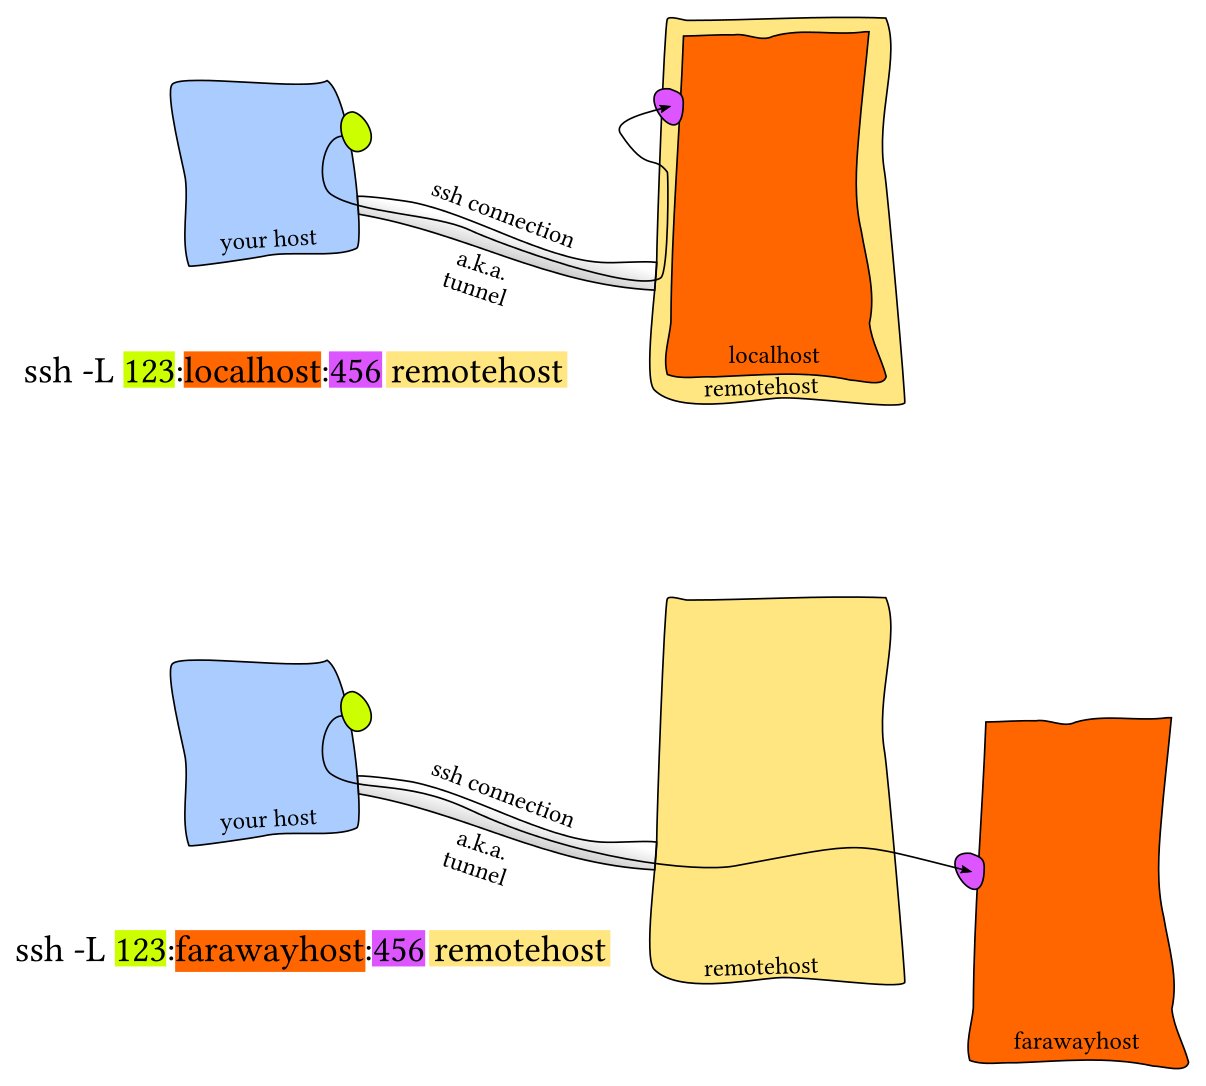
\includegraphics[width=160mm, scale=0.75]{pictures/local-port-forwarding.png}
 \caption{Local Port Forwarding}
\end{figure}

\subsubsection{Remote Port Forwarding}
\begin{figure}[H]
 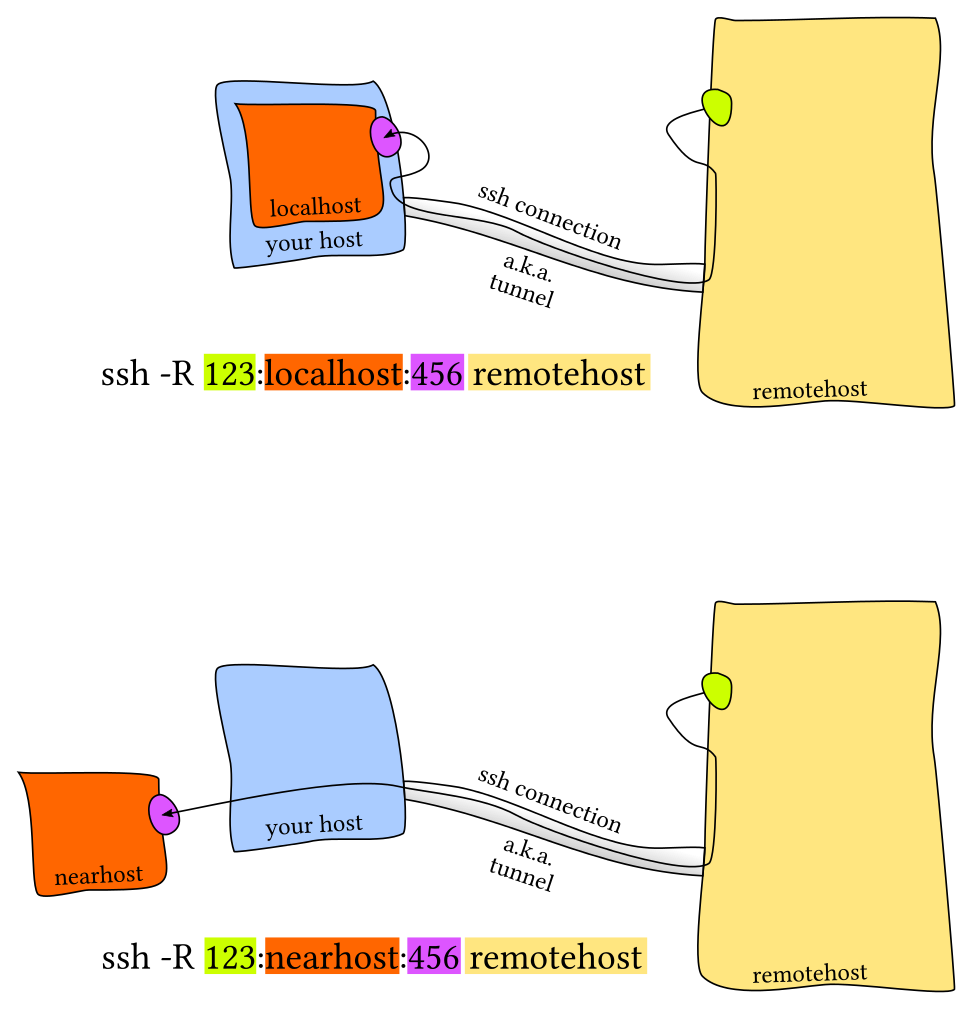
\includegraphics[width=160mm, scale=0.75]{pictures/remote-port-forwarding.png}
 \caption{Remote Port Forwarding}
\end{figure}

\subsubsection{SSH Configuration}

\begin{description}
 \lstitem{\~/.ssh/config} Dotfile used to configure \lstinline{ssh}. Also readable by other programs like \lstinline{scp}, \lstinline{rsync}, etc that can convert the settings into the corresponding flags
 \lstitem{/etc/ssh/sshd_config} Used for server side configuration. Can make changes like disabling password authentication, changing ssh ports, enabling X11 forwarding, etc. Can also specify config settings on a per user basis
\end{description}

\begin{itemize}
 \item Note: \lstinline{~/.ssh/config} has some potentially private info that you might not want to share with other people
\end{itemize}

\subsubsection{Miscellaneous SSH Stuff}

\begin{description}
 \lstitem{mosh} mobile shell that improves upon \lstinline{ssh} by allowing roaming connections, intermittent connectivity, and providing intelligent local echo
 \lstitem{sshfs} mounts a folder on a remote server locally, allowing you to use a local editor
\end{description}

\subsection{Bash vs Zsh}
\begin{itemize}
 \item \lstinline{bash} is the most common shell and is the default option on most shells
\end{itemize}

\begin{description}
 \lstitem{zsh} a superset of \lstinline{bash} that provides extra features like
\end{description}

\begin{itemize}
 \item Smarter globbing, \lstinline{**}
 \item Inline globbing/wildcard expansion
 \item Spelling correction
 \item Better tab completion/selection
 \item Path expansion (\lstinline{cd /u/lo/b} expands to \lstinline{/usr/local/bin})
\end{itemize}

\section{Version Control (Git)}

\subsection{Version Control Systems}
\begin{description}
 \item[Version Control Systems (VCS)]: tools to track changes to source code; maintain history of changes and improve collaboration
\end{description}

\subsection{Git's Data Model}

\subsubsection{Snapshots (commits)}
\begin{itemize}
 \item Git models history of a collection of files and folders inside a top-level directory as a series of snapshots (commits)
\end{itemize}

\begin{description}
 \item[blob]: a file in Git
 \item[tree]: a directory; maps names to blobs or trees (directories can contain other directories)
 \item[commit]: a snapshot of the top-level tree being tracked
\end{description}

\begin{lstlisting}
  <root> (tree) # top level directory
  |
  +- foo (tree)
  |  |
  |  + bar.txt (blob, contents = "hello world")
  |
  +- baz.txt (blob, contents = "git is wonderful")
\end{lstlisting}

\subsubsection{Git's model of history}
\begin{itemize}
 \item Git models history as a directed acyclic graph (DAG) of snapshots
 \item i.e. each snapshot in Git refers to a set of "parents" (older snapshots before it)
 \item Snapshots can have multiple parents (a set of parents) because a snapshot might descend from multiple parents
 \item ex. combining (merging) two parallel branches of development (2 parents)
\end{itemize}


\begin{lstlisting}
  # example of branching (newer commits on the right)
  o <-- o <-- o <-- o
            ^
             \
              --- o <-- o
\end{lstlisting}

\begin{itemize}
 \item The circle \lstinline{o}'s refer to individual commits (snapshots of entire tree)
 \item Note: the arrows point to the parent of each commit (i.e. the previous commits) and the newer commits are on the right
 \item After third commit, the history branches into 2 separate branches (ex. 2 separate features independently developed in parallel)
 \item Can later merge parallel branches to create a new snapshot with both features
\end{itemize}

\begin{lstlisting}
  # merging parallel branches in Git
  o <-- o <-- o <-- o <---- o
            ^            /
             \          v
              --- o <-- o
\end{lstlisting}

\begin{itemize}
 \item Git commits are immutable
 \item i.e. "edits" to the commit history actually add new commits instead of changing old commits
 \item References are then updated to point to new ones
\end{itemize}


\subsubsection{Data Model in pseudocode}

\begin{lstlisting}[language=c++]
  // a file is a bunch of bytes
  type blob = array<byte>

  // a directory contains named files and directories
  type tree = map<string, tree | file>

  // a commit has parents, metadata, and the top-level tree
  type commit = struct {
    parent: array<commit>
    author: string
    message: string
    snapshot: tree
  }
\end{lstlisting}


\subsubsection{Objects and content-addressing}
\begin{description}
 \item[object] a blob, tree, or commit
\end{description}

\begin{lstlisting}[language=c++]
  type object = blob | tree | commit
  // these objects are all content-addressed and given a SHA-1 hash
\end{lstlisting}

\begin{itemize}
 \item In Git's data store, all objects are content-addressable by their SHA-1 hash (160-bit string or 40 chars of hexadecimal)
\end{itemize}

\begin{lstlisting}
  objects = map<string, object>

  def store(object):
    id = sha1(object)
    objects[id] = object

  def load(id):
    return objects[id]
\end{lstlisting}

\begin{itemize}
 \item Since blobs, trees, and commits are all objects they can reference other objects by their hash
 \item i.e. don't have to contain the on-disk representation of the referenced object
\end{itemize}

\begin{description}
 \lstitem{git cat-file -p <SHA-1 hash>} visualizes the object pointed to by the hash
\end{description}

\subsubsection{References}
\begin{itemize}
 \item All snapshots can be identified by their SHA-1 hash but for convenience, can make human-readable references
\end{itemize}

\begin{description}
 \item[references]: human-readable pointers to commits (mutable)
       \lstitem{master}: a reference that usually points to the latest commit in the main development branch. Created by default when you init a git repo
       \lstitem{HEAD}: a reference that points to "where we currently are" in history. Allows you compare current position with other snapshots in history
\end{description}

\begin{itemize}
 \item Note: references are mutable (can point to other objects) but objects are immutable
 \item Can't change where hashes point to because the hash is determined from the object (which is immutable)
\end{itemize}

\begin{lstlisting}
  references = map<string, string>

  def update_reference(name, id):
    references[name] = id

  def read_reference(name):
    return references[name]

  def load_reference(name_or_id):
    if name_or_id in references:
        return load(references[name_or_id])
    else:
        return load(name_or_id)
\end{lstlisting}

\subsubsection{Repositories}
\begin{description}
 \item[repository] data storing \lstinline{objects} and \lstinline{references}
\end{description}

\begin{itemize}
 \item On disk, Git only stores objects and references
 \item All \lstinline{git} commands manipulate the commit DAG by adding objects and adding/updating references
\end{itemize}

\subsection{Staging Area}
\begin{description}
 \item[staging area] allows you to specify which code changes should be included in the next commit
\end{description}

\subsection{Git Command-Line Interface}

\subsubsection{Basics}
\begin{description}
 \lstitem{git help <command>} get help for a git command
 \lstitem{git init} creates a new git repo, with data stored in the .git directory
 \lstitem{git status} tells you what’s going on
 \lstitem{git add <filename>} adds files to staging area for next commit
 \lstitem{git commit} creates a new commit
 Write good commit messages!
 \lstitem{git log} shows a flattened log of history
 \lstitem{git log --all --graph --decorate --oneline} visualizes history as a DAG
 \lstitem{git diff <filename>} show differences since the last commit
 \lstitem{git diff <revision> <filename>} shows differences in a file between snapshots
 \lstitem{git diff --cached} show what changes are staged for next commit
 \lstitem{git checkout <revision>} updates HEAD and current branch. Changes files in working directory to match the revision snapshot (where HEAD now points to). Note that it throws any current uncommited changes
\end{description}

\subsubsection{Branching and Merging}
\begin{description}
 \lstitem{git branch} shows branches in repo
 \lstitem{git branch <name>} creates a branch. New branch points to the same current location in history (i.e. HEAD and new branch will resolve to same location)
 \lstitem{git checkout -b <name>} creates a branch and switches to it
 \begin{itemize}
  \item Equivalent to \lstinline{git branch <name>; git checkout <name>}
 \end{itemize}
 \lstitem{git merge <revision>} merges into current branch
 \lstitem{git mergetool} use a fancy tool to help resolve merge conflicts
 \lstitem{git merge --abort} aborts merge and puts you back in previous state before merge
 \lstitem{git merge --continue} finishes merge after merge conflict is resolved
 \lstitem{git rebase} rebase set of patches onto a new base
\end{description}

\begin{description}
 \item[fast forward]: if you merge a branch that has the the current commit (HEAD) as a predecessor, it will just move the references up to the merged branch (because no other changes required)
 \item[Merge conflicts]: when you merge parallel branches, Git may get confused if you have contradictory changes
\end{description}

\begin{itemize}
 \item For merge conflict, git will add conflict markers in the affected files to show incompatible code between the branches being merged
\end{itemize}

\subsubsection{Remotes}
\begin{itemize}
 \item Remotes used to collaborate with other people
 \item \lstinline{.git} folder contains entire repo history (objects, references, previous commits)
 \item Each person maintains their own copy of the git repo and they pass changes around with commits
 \item Remote repo (ex. GitHub) usually called \lstinline{origin}
\end{itemize}

\begin{description}
 \lstitem{git remote}list remotes
 \lstitem{git remote add <name> <url>} add a remote. Makes local repo aware of remote repo's
 \lstitem{git push <remote> <local branch>:<remote branch>} send objects to remote, and update remote reference
 \lstitem{git branch --set-upstream-to=<remote>/<remote branch>} set up correspondence between local and remote branch. Can then use shortened form \lstinline{git push}
 \lstitem{git fetch} retrieve objects/references from a remote
 \lstitem{git pull} same as \lstinline{git fetch; git merge}
 \lstitem{git clone} download repository from remote
\end{description}

\subsubsection{Undo}
\begin{description}
 \lstitem{git commit --amend} edit a commit’s contents/message
 \lstitem{git reset HEAD <file>} unstage a file
 \lstitem{git checkout -- <file>} discard changes
\end{description}

\subsubsection{Advanced Git}
\begin{description}
 \lstitem{git config} customize Git; can also directly edit \lstinline{~/.gitconfig}
 \lstitem{git clone --shallow} clone without entire version history (faster). Useful for big projects with many commits
 \lstitem{git add -p} interactive staging
 \lstitem{git rebase -i} interactive rebasing
 \lstitem{git blame} show who last edited which line
 \lstitem{git stash} temporarily remove modifications to working directory
 \lstitem{git stash pop} restore changes from \lstinline{git stash}
 \lstitem{git bisect} binary search history (e.g. failed unit tests)
 \lstitem{.gitignore} file used to specify intentionally untracked files to ignore
\end{description}


\section{Debugging and Profiling}

\subsection{Printf debugging and logging}
\begin{description}
 \item[printf debugging]: put print statements in code
 \item[logging]: create logs when some events happen. Can define severity levels (ex. INFO, DEBUG, WARN, ERROR, etc) and record when events/errors occur
\end{description}
\begin{itemize}
 \item Printf debugging can give a lot of output (not always desirable)
 \item Logging allows you to filter output based on severity level
 \item Logging can also be stored in files, sockets, or remote servers instead of STDOUT
 \item Most programs write their logs under \lstinline{/var/log}
\end{itemize}

\begin{description}
 \item[system log]: centralized log used in most Linux systems
       \lstitem{systemd} a Linux system daemon (runs in background) that controls many things like when services are enabled and running. Stores its log in \lstinline{/var/log/journal} in a specialized format
       \lstitem{journalctl} display logs from \lstinline{systemd}
       \lstitem{/var/log/system.log} centralized log used in macOS
       \lstitem{log show} displays system log in macOS
       \lstitem{dmesg}: UNIX command ot access kernel log
       \lstitem{logger} shell program to write to system logs
       lstitem{lnav}: CLI tool to help navigate log files
\end{description}

\begin{lstlisting}
  # Write to system log
  logger "Hello Logs"

  # Check log on macOS
  log show --last 1m | grep Hello

  # Check log on Linux
  journalctl --since "1m ago" | grep Hello
\end{lstlisting}

\subsection{Debuggers}
\begin{description}
 \item[debugger]: program that lets you interact with the execution of a program to find issues
       \lstitem{pdb}: Python Debugger
       \lstitem{ipdb}: improved \lstinline{pdb} using \lstinline{IPython} with tab completion, syntax highlighting, better tracebacks, and better introspection but same \lstinline{pdb} interface
\end{description}

\begin{description}
 \lstitem{gdb} debugger optimized for C-like language debugging that lets you probe any process and get its current machine state (registers, stack, program counter)
 \lstitem{pwndbg} better version of \lstinline{gdb}
 \lstitem{lldb} another better version of \lstinline{gdb}
\end{description}


\begin{itemize}
 \item Debugger features
       \begin{enumerate}
        \item Halt execution of the program when it reaches a certain line
        \item Step through the program one instruction at a time
        \item Inspect values of variables after the program crashed
        \item Conditionally halt the execution when a given condition is met
       \end{enumerate}
 \item Most programming languages have their own debugger
\end{itemize}

\subsubsection{Python Debugger (pdb) commands}
\begin{itemize}
 \item \textbf{l}(ist): Displays 11 lines around the current line or continue the previous listing
 \item \textbf{s}(tep): Execute the current line, stop at the first possible occasion
 \item \textbf{restart}: restart execution from beginning
 \item \textbf{n}(ext): Continue execution until the next line in the current function is reached or it returns
 \item \textbf{c}(ontinue): Continue until you reach the issue
 \item \textbf{b}(reak): Set a breakpoint (depending on the argument provided)
 \item \textbf{p}(rint): Evaluate the expression in the current context and print its value (ex. \lstinline{p arr} prints value of the array \lstinline{arr}). There’s also \lstinline{pp} to display using \lstinline{pprint} instead.
 \item \textbf{p locals()}: Prrints all current values
 \item \textbf{r}(eturn): Continue execution until the current function returns
 \item \textbf{q}(uit): Quit the debugger
\end{itemize}

\begin{lstlisting}
  python3 -m pdb script.py # run python debugger
\end{lstlisting}

\subsection{Debugging binary files}

\begin{itemize}
 \item Can even debug a binary file
 \item Whenever programs need to perform actions that only the kernel can, they make \textbf{System Calls} (syscalls)
\end{itemize}

\begin{description}
 \lstitem{strace} track syscalls in Linux
 \lstitem{dtrace} track syscalls in macOS or BSD
 \lstitem{dtruss} wrapper for \lstinline{dtrace} that has an interface similar to \lstinline{strace}
 \lstitem{lstat} a syscall that checks properties of files
\end{description}

\begin{lstlisting}
  # analyzing ls using strace on Linux
  sudo strace -e lstat ls -l > /dev/null
  4
  # analyzing ls using dtruss on macOS
  sudo dtruss -t lstat64_extended ls -l > /dev/null
\end{lstlisting}

\begin{description}
 \lstitem{tcpdump}: network packet analyzer that lets you read contents of network packets and filter them based on different criteria
\end{description}

\begin{itemize}
 \item Chrome/Firefox developer tools are useful for web development
       \begin{enumerate}
        \item Source code: inspect HTML/CSS/JS source code of any website
        \item Live HTML, CSS, JS modification: change the website content, styles and behavior to test
        \item Javascript shell: execute commands using the JS REPL
        \item Network: analyze the requests timeline.
        \item Storage: Look into the Cookies and local application storage.
       \end{enumerate}
\end{itemize}

\subsection{Static Analysis}
\begin{description}
 \item[static analysis]: take source code and analyze it using the language rules to find bugs
       \lstitem{pyflakes} python static analysis tool
       \lstitem{mypy} python tool that does type checking
       \lstitem{shellcheck} static analysis tool for shell scripts
 \item[code linting] using static analysis tools within editor or IDE
 \item[code formatters] autoformat code to be consistent with common styles/patterns for the language
\end{description}

\subsection{Profiling}
\begin{description}
 \item[profiler] software used to analyze code to find parts that take the most time and/or resources (for optimization)
\end{description}

\subsubsection{Timing}
\begin{description}
 \item[Real time]: elapsed time from start to finish. Includes time taken by other processes and time taken while blocked (ex. waiting for I/O or network)
 \item[User time]: time spent in CPU running user code
 \item[Sys time]: time spent in CPU running kernel code
\end{description}

\begin{itemize}
 \item Usually, \textbf{User + Sys} tells you how much time a process actualy spent in the CPU
\end{itemize}

\begin{lstlisting}
  time curl https://missing.csail.mit.edu &> /dev/null`
  real    0m2.561s
  user    0m0.015s
  sys     0m0.012s
  # have a slow connection so request takes 2 seconds but actually
  # only used 15ms of CPU user time and 12ms of kernel CPU time
\end{lstlisting}

\subsubsection{CPU profilers}
\begin{description}
 \item[tracing profiler]: keeps a record of very function call the program makes
 \item[sampling profiler]: probes your program periodically (usually every millisecond) and records the program's stack. Then presents aggregate statistics of the most time consuming tasks
\end{description}
\begin{itemize}
 \item CPU profilers are either tracing profilers or sampling profilers
 \item Sampling profilers are useful because they have less overhead
\end{itemize}

\begin{description}
 \lstitem{cProfile} Python tracing profiler
\end{description}

\begin{lstlisting}
python -m cProfile -s tottime grep.py 1000

[omitted program output]

 ncalls  tottime  percall  cumtime  percall filename:line(function)
     8000    0.266    0.000    0.292    0.000 {built-in method io}
     8000    0.153    0.000    0.894    0.000 grep.py:5(grep)
    93000    0.030    0.000    0.141    0.000 re.py:231(compile)
    17000    0.019    0.000    0.029    0.000 codecs.py:318(decode)
        1    0.017    0.017    0.911    0.911 grep.py:3(<module>)

[omitted lines]
\end{lstlisting}

\begin{description}
 \item[line profiler]: displays profiling information per line of code
       \lstitem{kernprof} Python line profiler
\end{description}

\begin{lstlisting}
$ kernprof -l -v a.py
Wrote profile results to urls.py.lprof
Timer unit: 1e-06 s

Total time: 0.636188 s
File: a.py
Function: get_urls at line 5

Line #  Hits         Time  Per Hit   % Time  Line Contents
==============================================================
5                                           @profile
6                                           def get_urls():
7       1     613909.0 613909.0    96.5  response=requests.get(url)
9       1          2.0      2.0     0.0  urls = []
10      25        685.0     27.4    0.1  for url in s.find('a'):
11      24         33.0      1.4    0.0  urls.append(url)
\end{lstlisting}

\subsubsection{Memory profilers}
\begin{description}
 \item[Valgrind] tool to identify memory leaks in C, C++
\end{description}

\begin{itemize}
 \item Note: even in garbage collected languages like Python, it is still useful to use a memory profiler becauses as long as you have pointers ot objects in memory, they won't be garbage collected.
\end{itemize}

\begin{lstlisting}
  $ python -m memory_profiler example.py
  Line #    Mem usage  Increment   Line Contents
  ==============================================
     3                           @profile
     4      5.97 MB    0.00 MB   def my_func():
     5     13.61 MB    7.64 MB       a = [1] * (10 ** 6)
     6    166.20 MB  152.59 MB       b = [2] * (2 * 10 ** 7)
     7     13.61 MB -152.59 MB       del b
     8     13.61 MB    0.00 MB       return a
\end{lstlisting}

\subsection{Event Profiling}
\begin{description}
 \lstitem{perf} reports system events related to your programs. Useful to detect poor cache locality, high amounts of pagefaults or livelocks.
 \lstitem{perf list} list events that can be traced with perf
 \lstitem{perf stat COMMAND ARG1 ARG2} gets counts of different events related to a process or command
 \lstitem{perf record COMMAND ARG1 ARG2}: records the run of a command and saves the statistical data into a file called \lstinline{perf.data}
 \lstinline{perf report}: formats and prints the data collected in \lstinline{perf.data}
\end{description}

\subsection{Profiler Visualization}
\begin{description}
 \item[Flame graph]: displays a hierarchy of function calls along the Y axis and time taken proportional to the X axis
 \item[Call graphs/control flow graphs] display the relationships between subroutines within a program by including functions as nodes and function calls between them as directed edges. Useful for studying flow of a program
       \lstitem{pycallgraph} Python library to generate call graphs
\end{description}

\subsection{Resource Monitoring}
\subsubsection{General monitoring}
\begin{description}
 \lstitem{htop} shows different stas for currently running processes on the system
 \lstitem{dstat} computes real-time resource metrics for different subsystems like I/O, networking, CPU utilization, context switches, etc
\end{description}

\subsubsection{I/O operations}
\begin{description}
 \lstitem{iotop} displays live I/O usage information and is handy to check if a process is doing heavy I/O disk operations
\end{description}

\subsubsection{Disk Usage}
\begin{description}
 \lstitem{df -h} displays metrics per partitions
 \lstitem{du -h} displays disk usage per file for the current directory
 \lstitem{ncdu} interactive version of \lstinline{du} that lets you navigate folders and delete stuff as you navigate
\end{description}

\subsubsection{Memory Usage}
\begin{description}
 \lstitem{free} displays total moutn fo free and used memory in the system
\end{description}

\subsubsection{Open Files}
\begin{description}
 \lstitem{lsof} lists info about files opened by processes
\end{description}

\subsubsection{Network Connections and Config}
\begin{description}
 \lstitem{ss} lets you monitor incoming and outgoing network packets statistics as well as interface statistics. Commonly used to figurr out what process is using a given port in a machine
 \lstitem{ip} displays routing, network devices and interfaces
\end{description}

\subsubsection{Network Usage}
\begin{description}
 \lstitem{nethog} interactive CLI tool for monitoring network usage
\end{description}

\subsection{Benchmarking}
\begin{itemize}
 \item Benchmarking is used to compare software to see which one is better for specific use cases
\end{itemize}

\begin{description}
 \lstitem{hyperfine} benchmarking tool for ommand line programs
\end{description}

\begin{lstlisting}
  $ hyperfine --warmup 3 'fd -e jpg' 'find . -iname "*.jpg"'
  Benchmark #1: fd -e jpg
  Time (mean +- STDEV):      51.4 ms +-   2.9 ms
  [User: 121.0 ms, System: 160.5 ms]
  Range (min ... max):    44.2 ms ...  60.1 ms    56 runs

  Benchmark #2: find . -iname "*.jpg"
  Time (mean +- STDEV):      1.126 s +-  0.101 s
  [User: 141.1 ms, System: 956.1 ms]
  Range (min ... max):    0.975 s ...  1.287 s    10 runs

  Summary
  'fd -e jpg' ran
   21.89 +- 2.33 times faster than 'find . -iname "*.jpg"'
\end{lstlisting}




\section{Metaprogramming}

\subsection{Build Systems}

\begin{description}
 \item[Build system]: automates building process to convert inputs (dependencies) to outputs (targets) using specified rules
       \lstitem{make} most common build system on UNIX. Good for simple to medium complexity
       \lstitem{cmake} another build system that is opinionated and optimized for specific tasks
       \lstitem{Makefile} files used to specify dependencies, targets, and rules for \lstinline{make}
\end{description}

\begin{itemize}
 \item Build system aims to do minimal work
 \item i.e. if a dependency has not changed, it will not rebuild the associated targets
\end{itemize}

\begin{lstlisting}
  # first directive
  paper.pdf: paper.tex plot-data.png
    pdflatex paper.tex

  # second directive
  plot-%.png: %.dat plot.py
    ./plot.py -i $*.dat -o $@
\end{lstlisting}

\begin{description}
 \item[Directive]: rule for producing target (left-hand side of colon \lstinline{:})  using the dependencies (right-hand side of colon \lstinline{:})
 \item[Target]: desired output (ex. pdf, mp4)
 \item[Dependency]: software that is required to built the target
 \item[Rule]: specifies how to get target from dependencies (ex. run a \lstinline{python} file or \lstinline{pdflatex})
\end{description}

\begin{itemize}
 \item The indented block in each directive is a sequence of programs to produce the target from the dependencies
 \item Note: first directive in \lstinline{make} defines teh default goal (what is built when you run \lstinline{make} with no arguments)
 \item Can also build specific targets with arguments: \lstinline{make plot-data.png}
 \item Note: \lstinline{Makefile} requires tabs for the rules; spaces will not work
\end{itemize}

\begin{description}
 \lstitem{\%} wildcard that specifies "patterns" in a rule and matches the same string on the left and on the right
 \lstitem{\$*} special variable that matches \lstinline{%}
 \lstitem{\$@} special variable for target
\end{description}

\begin{itemize}
 \item ex. if the target \lstinline{plot-foo.png} is requested, \lstinline{make} will look for the dependencies \lstinline{foo.dat} and \lstinline{plot.py}
 \item Note: if your \lstinline{Makefile} is super complicated, it probably means you should use \lstinline{cmake} or something else
 \item Can use \lstinline{make} at the top level and use it to call opinionated build systems like \lstinline{cmake}
\end{itemize}

\subsection{Versioning}
\begin{itemize}
 \item Versions are usually numerical and are used to ensure that software keeps working
 \item Helps users to determine what is compatible/incompatible when choosing which version of a dependency to install
\end{itemize}

\subsubsection{Semantic Versioning}

\begin{description}
 \item[Semantic versioning]: common version format of \textbf{major.minor.patch}
\end{description}

\begin{itemize}
 \item Semantic versioning rules
       \begin{enumerate}
        \item if API is \textbf{unchanged}, increase the \textbf{patch} version
        \item if API is changed (\textbf{backwards-compatible}), increase the \textbf{minor} version (reset patch version to 0)
        \item if API is changed (\textbf{non-backwards-compatible}), increase \textbf{major} version (reset minor and patch version to 0)
       \end{enumerate}
 \item Specify dependencies with major and minor version numbers
 \item Can use any version of dependency with the same major and same or higher minor version
 \item Usually patch updates are for security fixes; the software will still run, but you might still want to update it
 \item The best type of dependency is when you depend on version X.0.0 because you can use any minor or patch version from major version X
 \item Python 2 and Python 3 are an example of a major version bump (incompatible code)
\end{itemize}

\subsubsection{Lock files}

\begin{description}
 \item[lock file]: file that lists the exact version you are currently depending on of each dependency. Dependencies are then only updated when you run the update program
 \item[vendoring]: explicitly copy all the code of your dependencies in your own project. Gives you total control over any changes, but makes updating difficult
\end{description}

\begin{itemize}
 \item Lock files are useful because they avoid unnecessary recompiles, having reproducible builds, and avoid automatically updating to potentially faulty versions
\end{itemize}

\subsection{Continuous integration systems}
\begin{description}
 \item[Continuous integration (CI)]: software (cloud build system) that runs whenver code changes
\end{description}

\begin{itemize}
 \item Continuous integration can be general or specific to certain tasks (ex. run test suite after a code push)
 \item ex. dependabot is CI tool that scans a repository for newer versions of dependencies
 \item ex. GitHub pages is another CI action that runs the Jekyll static site generator on every push to \lstinline{master} and loads the built site on a particular domain
 \item CI software usually give badges that you can add to README
\end{itemize}

\subsection{Testing}
\begin{description}
 \item[Test suite]: collective term for all the tests
 \item[Unit test]: a "micro-test" that tests a specific feature in isolation
 \item[Integration test]: a "macro-test" that tests if different features/components work together properly
 \item[Regression test]: test that implements a specific pattern that previously caused a bug to ensure that the bug does not reappear
 \item[Mocking]: replace a function, module, or type with a dummy implementation to avoid testing unrelated functionality
\end{description}

\section{Security and Cryptography}

\subsection{Entropy}
\begin{description}
 \item[Entropy]: measure of randomness. Useful to determine strength of a password
\end{description}

\begin{itemize}
 \item Entropy is measured in bits
 \item Time required to brute force a password is proportional to its bits of entropy
 \item For random uniform selection from a set of possible outcomes, entropy is calculated as
       \begin{align}
        \text{Entropy} = log_2(\text{\# of possibilities})
       \end{align}
 \item ex. fair coin flip has $\text{Entropy} = log_2(2) = 1$ bit of entropy
 \item ex. dice roll (6-sided die) has $\text{Entropy} = log_2(6) \approx 2.58$ bit of entropy
 \item Heuristic: $\sim 40$ bits of entropy is pretty good for online guessing and $\sim 80$ bits of entropy is pretty resistant to offline guessing
\end{itemize}

\subsection{Hash Functions}
\begin{description}
 \item[Cryptographic hash function (CHF)]: maps data of arbitrary size to a fixed size
\end{description}

\begin{lstlisting}
  hash(value: array<byte>) -> vector<byte, N>  (for some fixed N)
\end{lstlisting}


\begin{itemize}
 \item ex. SHA-1 is a hash function used in Git. It maps arbitary-sized inputs to 160-bit outputs (40 hexadecimal characters)
\end{itemize}

\begin{description}
 \lstitem{sha1sum} apply SHA-1 hash to an input
\end{description}

\begin{lstlisting}
$ printf 'hello' | sha1sum
aaf4c61ddcc5e8a2dabede0f3b482cd9aea9434d
$ printf 'hello' | sha1sum
aaf4c61ddcc5e8a2dabede0f3b482cd9aea9434d
$ printf 'Hello' | sha1sum
f7ff9e8b7bb2e09b70935a5d785e0cc5d9d0abf0

# Note: the SHA-1 hash is deterministic (same output for same input)
# and very sensitive to small changes (i.e. collision resistant)
\end{lstlisting}

\subsubsection{Properties of Cryptographic Hash Functions}
\begin{itemize}
 \item A hash function is a hard-to-invert random-looking (but deterministic) function with these properties
       \begin{itemize}
        \item \textbf{Deterministic}: same input always generates same output
        \item \textbf{Non-invertible}: hard to find an input \lstinline{m} such that \lstinline{hash(m) = h} for some desired output \lstinline{h}
        \item \textbf{Target collision resistant}: given an input \lstinline{m_1}, it’s hard to find a different input \lstinline{m_2} such that \lstinline{hash(m_1) = hash(m_2)}
        \item \textbf{Collision resistant}: hard to find two inputs \lstinline{m_1} and \lstinline{m_2} such that \lstinline{hash(m_1) = hash(m_2)} (note that this is a strictly stronger property than target collision resistance)
       \end{itemize}
\end{itemize}


\subsection{Applications of Cryptographic Hash Functions}
\subsubsection{Content-addressed storage (Git)}
\begin{itemize}
 \item Hash is a "summary of a file"
 \item To avoid collisions (commits, files, other objects are all addressable with hashes), you use a cryptographic hash function because it is collision resistant
 \item i.e. won't have the same hash pointing to 2 different commits
\end{itemize}

\subsubsection{File Content Summary/Download Verification}
\begin{itemize}
 \item Software is often downloaded from untrusted mirrors (ex. Linux ISOs)
 \item The official sites usually post hashes along with the download links (pointing to third-party mirrors) so that the hash can be checked after downloading the file
\end{itemize}

\subsubsection{Commitment schemes}
\begin{itemize}
 \item Commitment schemes used when you want to commit to a particular value but reveal the value itself later
 \item Ex. for a fair coin toss "in my head" without a trusted share coin that both parties can see
 \item Coin flipper can choose a value \lstinline{r = random()} and then share \lstinline{h = sha256(r)}
 \item Guesser then guesses heads or tails based on if \lstinline{r} is even or odd
 \item After guesser calls, the flipper reveals the value \lstinline{r} and guesser verifies that cheating hasn't occurred by checking \lstinline{h == sha256(r)}
 \item Since hash function is noninvertible, it is also hard for the guesser to cheat by inverting the hash \lstinline{h}
\end{itemize}

\subsection{Key Derivation Functions (KDFs)}
\begin{description}
 \item[Key Derivation Functions (KDFs)]: deliberately slow to slow down offline brute-force attacks. Often for producing fixed-length output for use as keys in other cryptographic algorithms
 \item[PBKDF2]: Passowrd Base Key Derivation Function 2
 \item[Plain text]: message to be encrypted
 \item[Cypher text]: encrypted message
\end{description}

\subsubsection{Applications of Key Derivation functions}
\begin{enumerate}
 \item Producing keys from passphrases for use in other cryptographic algorithms (ex. symmetric cryptography)
 \item Storing login credentials
       \begin{itemize}
        \item Storing plaintext passwords is bad if database is comprised
        \item Instead generate and store both a random salt \lstinline{salt = random()} and  \lstinline{KDF(password + salt)}
        \item Then verify login temps by re-computing the KDF given the entered password and stored salt
        \item Fights against rainbow tables where people store the hashes of previously used passwords
       \end{itemize}
\end{enumerate}

\subsection{Symmetric Cryptography}
\begin{lstlisting}
keygen() -> key  (this function is randomized)

encrypt(plaintext: array<byte>, key) -> array<byte> (ciphertext)
decrypt(ciphertext: array<byte>, key) -> array<byte>  (plaintext)
\end{lstlisting}

\subsubsection{Properties of keygen(), encrypt(), decrypt() - Symmetric Cryptography}
\begin{enumerate}
 \item Invertibility: given the output (ciphertext), it is hard to determine the input (plaintext) without the key
 \item Correctness: \lstinline{decrypt(encrypt(m, k), k) = m}
\end{enumerate}

\subsubsection{Symmetric Cryptography Applications}
\begin{itemize}
 \item File encryption for storage in an untrusted cloud service
 \item Use KDFs to encrypt a file with a passphrase
 \item i.e. generate \lstinline{key = KDF(passphrase)} and then store \lstinline{encrypt(file, key)}
\end{itemize}

\subsection{Asymmetric Cryptography}
\begin{description}
 \item[Private key]: meant to be kept secret (used to unlock file)
 \item[Public key]: meant to be publicly shared and won't affect security (used to unlock file)
\end{description}

\begin{lstlisting}
keygen() -> (publickey, privatekey)  # this function is randomized

encrypt(plaintxt: array<byte>, publickey) -> array<byte> (ciphertxt)
decrypt(ciphertxt: array<byte>, privatekey) -> array<byte> (plaintxt)

sign(msg: array<byte>, privatekey) -> array<byte> (signature)
verify(msg: array<byte>, signature: array<byte>, publickey) -> bool
# bool indicates whether or not the signature is valid
\end{lstlisting}

\subsubsection{Properties of keygen(), encrypt(), decrypt() - Asymmetric Cryptography}
\begin{itemize}
 \item Invertibility: given the output (ciphertext), it's hard to determine the input (plaintext) without the private key
 \item Decryption correctness: \lstinline{decrypt(encrypt(msg, public key), private key) = msg}
 \item Hard to forge: for any message, without the private key, it's hard to produce a signature such that \lstinline{verify(message, signature, public key)}
 \item Verification correctness: \lstinline{verify(message, sign(message, private key), public key) = true}
\end{itemize}


\subsubsection{Applications of Asymmetric Cryptography}
\begin{itemize}
 \item PGP email encryption: people can have public keys posted online (in a PGP keyserver, or on Keybase) and then anyone can send them encrypted email
 \item Private messaging (Signal and Keybase): use asymmetric keys to establish private communication channels
 \item Signing software (Git): have GPG-signed commits and tags with a posted public key so anyone can verify authnticity of downloaded software
\end{itemize}

\subsection{Symmetric vs Asymmetric Cryptography}
\begin{itemize}
 \item For symmetric cryptography, there needs to be an initial exchange of keys (may or may not be possible)
       \begin{itemize}
        \item Because you need the same key to unlock and lock
       \end{itemize}
 \item But asymmetric cryptography avoids this problem because you can freely share the public key in an unsafe channel
       \begin{itemize}
        \item Because the key to lock (public key) is separete form the key to unlock (private key)
       \end{itemize}
\end{itemize}

\subsection{Key distribution}
\begin{itemize}
 \item For asymmetric cryptography, you need to reliably distribute public keys and map public keys to real-world identities
 \item i.e. figure out if person is pretending to be someone else and giving you the wrong public key
 \item Signal uses "trust on first use" (assume person is who they say they are until proven wrong) and supports out-of-band public key exchange (i.e. verify public keys in person)
 \item PGP uses "web of trust" where you have trusted introducers and you share certifying signatures along with your public key (i.e. hope that the receiver trusts one of those signatures that are"vouching" for you)
\end{itemize}

\subsection{Cryptography Case Studies}

\subsubsection{Password Managers}
\begin{itemize}
 \item Password managers use unique, randomly generated high-entorpy passwords for all your accounts
 \item Passwords are saved in one place and ecnrypted with a symmetric cipher with a key produced from a passphrase using a KDF
 \item This allows you to avoid password reuse (less impact when websites get compromised), use high-entropy passwords, and only requires you to remember a single high-entropy password
\end{itemize}

\subsubsection{Two-factor authentication (2FA)}
\begin{itemize}
 \item 2FA requires you to use a passphrase along with a 2FA authenticator in order to protect against stolen passowrds and phishing attacks
 \item i.e. something extra to verify that it's "actually you" and not someone who happens to know the passphrase
\end{itemize}

\subsubsection{Full disk encryption}
\begin{itemize}
 \item Entire disk on computer is encrypted with a symmetric cipher with a key protected by a passphrase
\end{itemize}

\subsubsection{Private messaging}
\begin{itemize}
 \item End-to-end security provided using asymmetric key encryption
 \item For public keys, either authenticate public keys out-of-band or trust social proofs
\end{itemize}

\subsubsection{SSH}
\begin{enumerate}
 \item User runs \lstinline{ssh-keygen} to generate an asymmetric key pair \lstinline{public_key, private_key}
       \begin{itemize}
        \item Public key is stored as plaintext
        \item Private key is encrypted on disk
        \item User also provides a passphrase which is fed into a key derivation function to produce a key which is then used to encrypt the private key with a symmetric cipher
       \end{itemize}
 \item Client's public key is stored on \lstinline{.ssh/authorized_keys} on the server
 \item During use, a conneting client can prove its identity using asymmetric signatures with challenge response
       \begin{enumerate}
        \item Server picks a random number and sends it to the client
        \item Client signs this message and sends the signature back to the server
        \item Server checks the signature against the public key on record
        \item This proves that the client has the private key corresponding to the public key that in the server's \lstinline{.ssh/authorized_keys} file
       \end{enumerate}
 \item User is given remote access
\end{enumerate}


\section{Miscellaneous}

\subsection{Daemons}
\begin{description}
 \item[Daemon]: series of processes that are always running the background. Often has a name ending with \lstinline{d}
       \lstitem{sshd} SSH daemon listens to SSH requrests and authenticates users
       \lstitem{systemd} system daemon in Linux that runs and sets up smaller daemon processes (ex. netowrk, screen, etc)
       \lstitem{systemctl status} list current running daemons
\end{description}

\begin{itemize}
 \item \lstinline{systemctl} command used to interact with \lstinline{systemd} in order to \lstinline{enable}, \lstinline{disable}, \lstinline{start}, \lstinline{stop}, \lstinline{restart}, or check \lstinline{status} of service/daemons
\end{itemize}

\begin{lstlisting}
# Create custom daemon to run simple Python app

# /etc/systemd/system/myapp.service
[Unit]
Description=My Custom App
After=network.target

[Service]
User=foo
Group=foo
WorkingDirectory=/home/foo/projects/mydaemon
ExecStart=/usr/bin/local/python3.7 app.py
Restart=on-failure

[Install]
WantedBy=multi-user.target
\end{lstlisting}

\begin{description}
 \lstitem{cron} daemon used by system to perform scheduled tasks. Can use \lstinline{cron} to run a program at a given frequency without making a custom daemon
\end{description}

\subsection{FUSE}
\begin{description}
 \item[FUSE]: Filesystem in User Space; allows filesystems to be implemented by a user space
\end{description}

\begin{itemize}
 \item UNIX systems only allow kernel to perform filesystem calls
 \item FUSE then allows user to implement arbitrary filesystem calls
 \item ex. FUSE can be used so that whenever you perform an operation in a virtual filesystem, that operation is forwarded through SSH to a remote machine, performed there, and the output is returned back to you
 \item This allows local programs to see the file as if it was in your computer while in reality it's on a remote server
\end{itemize}

\subsubsection{Examples of FUSE filesystems}
\begin{description}
 \lstitem{sshfs} open locally remote files/folder through an SSH connection
 \lstitem{rclone} mount cloud storage services like Dropbox, Google Drive, Amazon S3, or Google Cloud storage and open data locally
 \lstitem{gocryptfs} encrypted overlay system; files are stored encrypted but once the filesystem is mounted they appear as plaintext in the mountpoint
 \lstitem{kbfs} distributed filesystem with end-to-end encryption. You can have private, shared and public folders.
 \lstitem{borgbackup} mount your deduplicated, compressed and encrypted backups for ease of browsing
\end{description}

\subsection{APIs}
\begin{description}
 \lstitem{curl} fetch URL and give you response
 \lstitem{jq} JSON query tool
\end{description}
\begin{itemize}
 \item Most online APIs are structured URLs
 \item Often rooted at \lstinline{api.service.com} where the path and query parameters indicate which data you want to read or what action you want to perform
 \item Usually responses are formatted as JSON, which you can then pipe through a tool like \lstinline{jq} to view and manipulate
 \item Some APIs require authentication (usually OAuth) where you send a secret token with the request
 \item Note: the tokens "act as you" so they should be kept secret to avoid other people impersonating you
\end{itemize}

\subsection{Common command-line flags/patterns}
\begin{itemize}
 \item Most tools have a \lstinline{--help} flag to display brief instructions
 \item Destructive tools usually have a "dry run" flag where they only print what they would have done, but not actually do the change
 \item Also have an "interactive" \lstinline{-i} flag to prompt user
 \item Can use \lstinline{--version} or \lstinline{-V} to view the program version (useful for bug reporting)
 \item Usually have a \lstinline{--verbose} or \lstinline{-v} flag to produce more output (useful for debugging)
 \item The \lstinline{--quiet} flag makes the program only print stuff for errors
 \item Often, a dash \lstinline{-} in place of a file name means STDIN/STDOUT
 \item Possible destructive tools are generally not recursive by default but support a "recursive" flag \lstinline{-r}
 \item To pass somehting that looks like a flag as a normal argument, use double dashes \lstinline{--} to tell the program to stop processing flags and options
\end{itemize}

\subsection{VPNs}
\begin{itemize}
 \item Best case: VPN lets you "change your internet service provider"
 \item All your traffic will look like it's coming from the VPN provider instead of your "real location and the network you are connected to will only see encrypted traffic
 \item Note: VPNs just shift your trust from your current ISP to the VPN host
 \item Tradeoff may be worthwhile on an untrusted public network, but still a risk
 \item Also, most of your sensitive traffic is already encrypted through HTTPs or TLS
 \item i.e. network operator can only see what servers you access, but nothing in your data
 \item VPN providers can also be malicious/opportunist and log or sell your data
       "\end{itemize}

\subsection{Booting + Live USBs}
\begin{description}
 \item[BIOS]: Basic Input/Output System; firmware used to initialize hardware during booting process and to provide runtime services for OS and programs (first software to run)
 \item[Unified Extensible Firmware Interface (UEFI)]: specification for software interface between OS and platform firmware. UEFI replaces legacy IBO interface. Can support remote diagnostics and computer repair even with no OS installed
 \item[Live USBs] USB flash drive containing an OS. Helpful to recover data or fix the OS when operating system no longer boots (use live USB for other OS and mount old hard drive to access files)
\end{description}

\begin{itemize}
 \item When machine boots up, before the OS is loaded, the BIOS/UEFI initializes the system
 \item Can enter specific key combo to configure BIOS/UEFI and change hardware-related settings
 \item Also have key combos to enter boot menu to boot from alternative devices (ex. live USB) instead of hard drive
\end{itemize}

\subsection{Docker, Vagrant, VMs, Cloud, Openstack}
\begin{description}
 \item[Virtual machines]: emulator for a whole computer system (including OS). Useful for isolated environment to test, develop, or explore (run potentially malicious code)
 \item[vagrant] tool to define machine configs (OS, services, packages, etc) in code, and then instantiate VMs with \lstinline{vagrant up}
 \item[Docker] tool like \lstinline{vagrant} but uses containers instead of VMs.
\end{description}

\begin{itemize}
 \item Can also rent VMs on the cloud
 \item Gives you instant access to a cheap always-on public IP address with lots of CPU, disk, RAM, and/or GPU
\end{itemize}








\end{document}
